% Dieser Text ist urheberrechtlich gesch\"utzt
% Er stellt einen Auszug eines von mir erstellten Referates da
% und darf nicht gewerblich genutzt werden
% die private bzw. Studiums bezogen Nutzung ist frei
% April 2011
% Autor: Sascha Frank 
% Universit\"at Freiburg 
% www.informatik.uni-freiburg.de/~frank/
% frank < was da sonst immer steht > tf.uni-freiburg.de
\documentclass[hyperref={pdfpagelabels=false}]{beamer}
% Die Hyperref Option hyperref={pdfpagelabels=false} verhindert die Warnung:
% Package hyperref Warning: Option `pdfpagelabels' is turned off
% (hyperref)                because \thepage is undefined. 
% Hyperref stopped early 
\usetheme{Warsaw}
\beamertemplatenavigationsymbolsempty
\usepackage[T1]{fontenc}
\usepackage[ngerman]{babel}
\usepackage[utf8]{inputenc}
\usepackage{amsmath,amsfonts,amssymb}
\usepackage{multimedia}
\usepackage{textcomp}
\usepackage{multirow}
\usepackage[sf,SF]{subfigure}
\usepackage{caption}
\usepackage{booktabs}
\usepackage{threeparttable}
\captionsetup[figure]{labelformat=empty}% redefines the caption setup of the figures environment in the beamer class.
\captionsetup[table]{labelformat=empty}% redefines the caption setup of the table environment in the beamer class.
\usepackage{upgreek}
\usepackage{lmodern}
% \usepackage{geometry}
% \usepackage[absolute,overlay]{textpos}
% Das Paket lmodern erspart die folgenden Warnungen:
% LaTeX Font Warning: Font shape `OT1/cmss/m/n' in size <4> not available
% (Font)              size <5> substituted on input line 22.
% LaTeX Font Warning: Size substitutions with differences
% (Font)              up to 1.0pt have occurred.
%
% Wenn \titel{\ldots} \author{\ldots} erst nach \begin{document} kommen,
% kommt folgende Warnung:
% Package hyperref Warning: Option `pdfauthor' has already been used,
% (hyperref) ... 
% Daher steht es hier vor \begin{document}
%\setbeamertemplate{headline}{} %%beseitigt Kopfzeile mit Kapitelübersicht und -navigation%%
%\setbeamertemplate{footline}{} %%beseitigt Fußzeile mit Namen und Titel%%
%\usepackage{biblatex}
%\bibliography{../Masterarbeit/Referenz}
\setbeamertemplate{footline}[frame number]
\setbeamerfont{frame number in foot}{size=\footnotesize}
% zusaetzlich ist das usepackage{beamerthemeshadow} eingebunden 
\usepackage{beamerthemeshadow}
% \beamersetuncovermixins{\opaqueness<1>{25}}{\opaqueness<2->{15}}
%  sorgt dafuer das die Elemente die erst noch (zukuenftig) kommen 
%  nur schwach angedeutet erscheinen 
% \beamersetuncovermixins{\opaqueness<1>{25}}{\opaqueness<2->{15}}
% klappt auch bei Tabellen, wenn teTeX verwendet wird\ldots
%\begin{document}
\newcommand\blfootnote[1]{%
  \begingroup
  \renewcommand\thefootnote{}\footnote{#1}%
  \addtocounter{footnote}{-1}%
  \endgroup
}

\begin{document}
\title{Water at $\upalpha$-Alumina Surfaces: Energetics, Dynamics and Kinetics}
\subtitle{{\bf Disputation}}   
\author{Sophia L. Heiden}
\institute{
\includegraphics[width=1.5cm]{figures/UP-Logo_Matjpg.jpg}}
% \date{\today} 
\date{18.03.2019}

\begin{frame}[plain]
 \addtocounter{framenumber}{-3}
\titlepage
\end{frame} 


\begin{frame}[plain]
% \addtocounter{framenumber}{0}
 \frametitle{Motivation}
 \begin{columns}[c]
  \column{0.5\textwidth}
  \begin{itemize}
   \item Surface science, heterogene Katalyse
   \item Computerbasierte Modellierung von Prozessen
  \end{itemize}
  \column{0.5\textwidth}
   \framebox{
   
\includegraphics[width=1.in]{figures/scientist-clipart-nerd.jpg}\tiny{$^1$} %https://mbtskoudsalg.com/images/scientist-clipart-nerd.jpg
   ~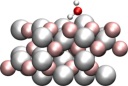
\includegraphics[width=1.in]{figures/surfaceprocess.pdf}}
 \end{columns}
 \blfootnote{\tiny{$^1$https://goo.gl/images/tXHjDc, $^2$https://goo.gl/images/kAcRcR}}%https://external-preview.redd.it/raUdEwh8-J01prs80mqdLGG-sVTfg-80YXxwnfwVRtY.jpg?s=eabf5472b6d7a49b7a66ebfecade4f2b9d49dc2f}}
 \pause
 \begin{columns}[c]
  \column{0.7\textwidth}
  Anwendungen von Al$_2$O$_3$
  \begin{itemize}
   \item Rubinlaser
   \item Katalysator: Clausprozess
   \item Keramisches Material
   \item Abgase von Festtreibstoffraketen $\rightarrow$ Probennahme schwierig
  \end{itemize}
  \column{0.3\textwidth}
   \framebox{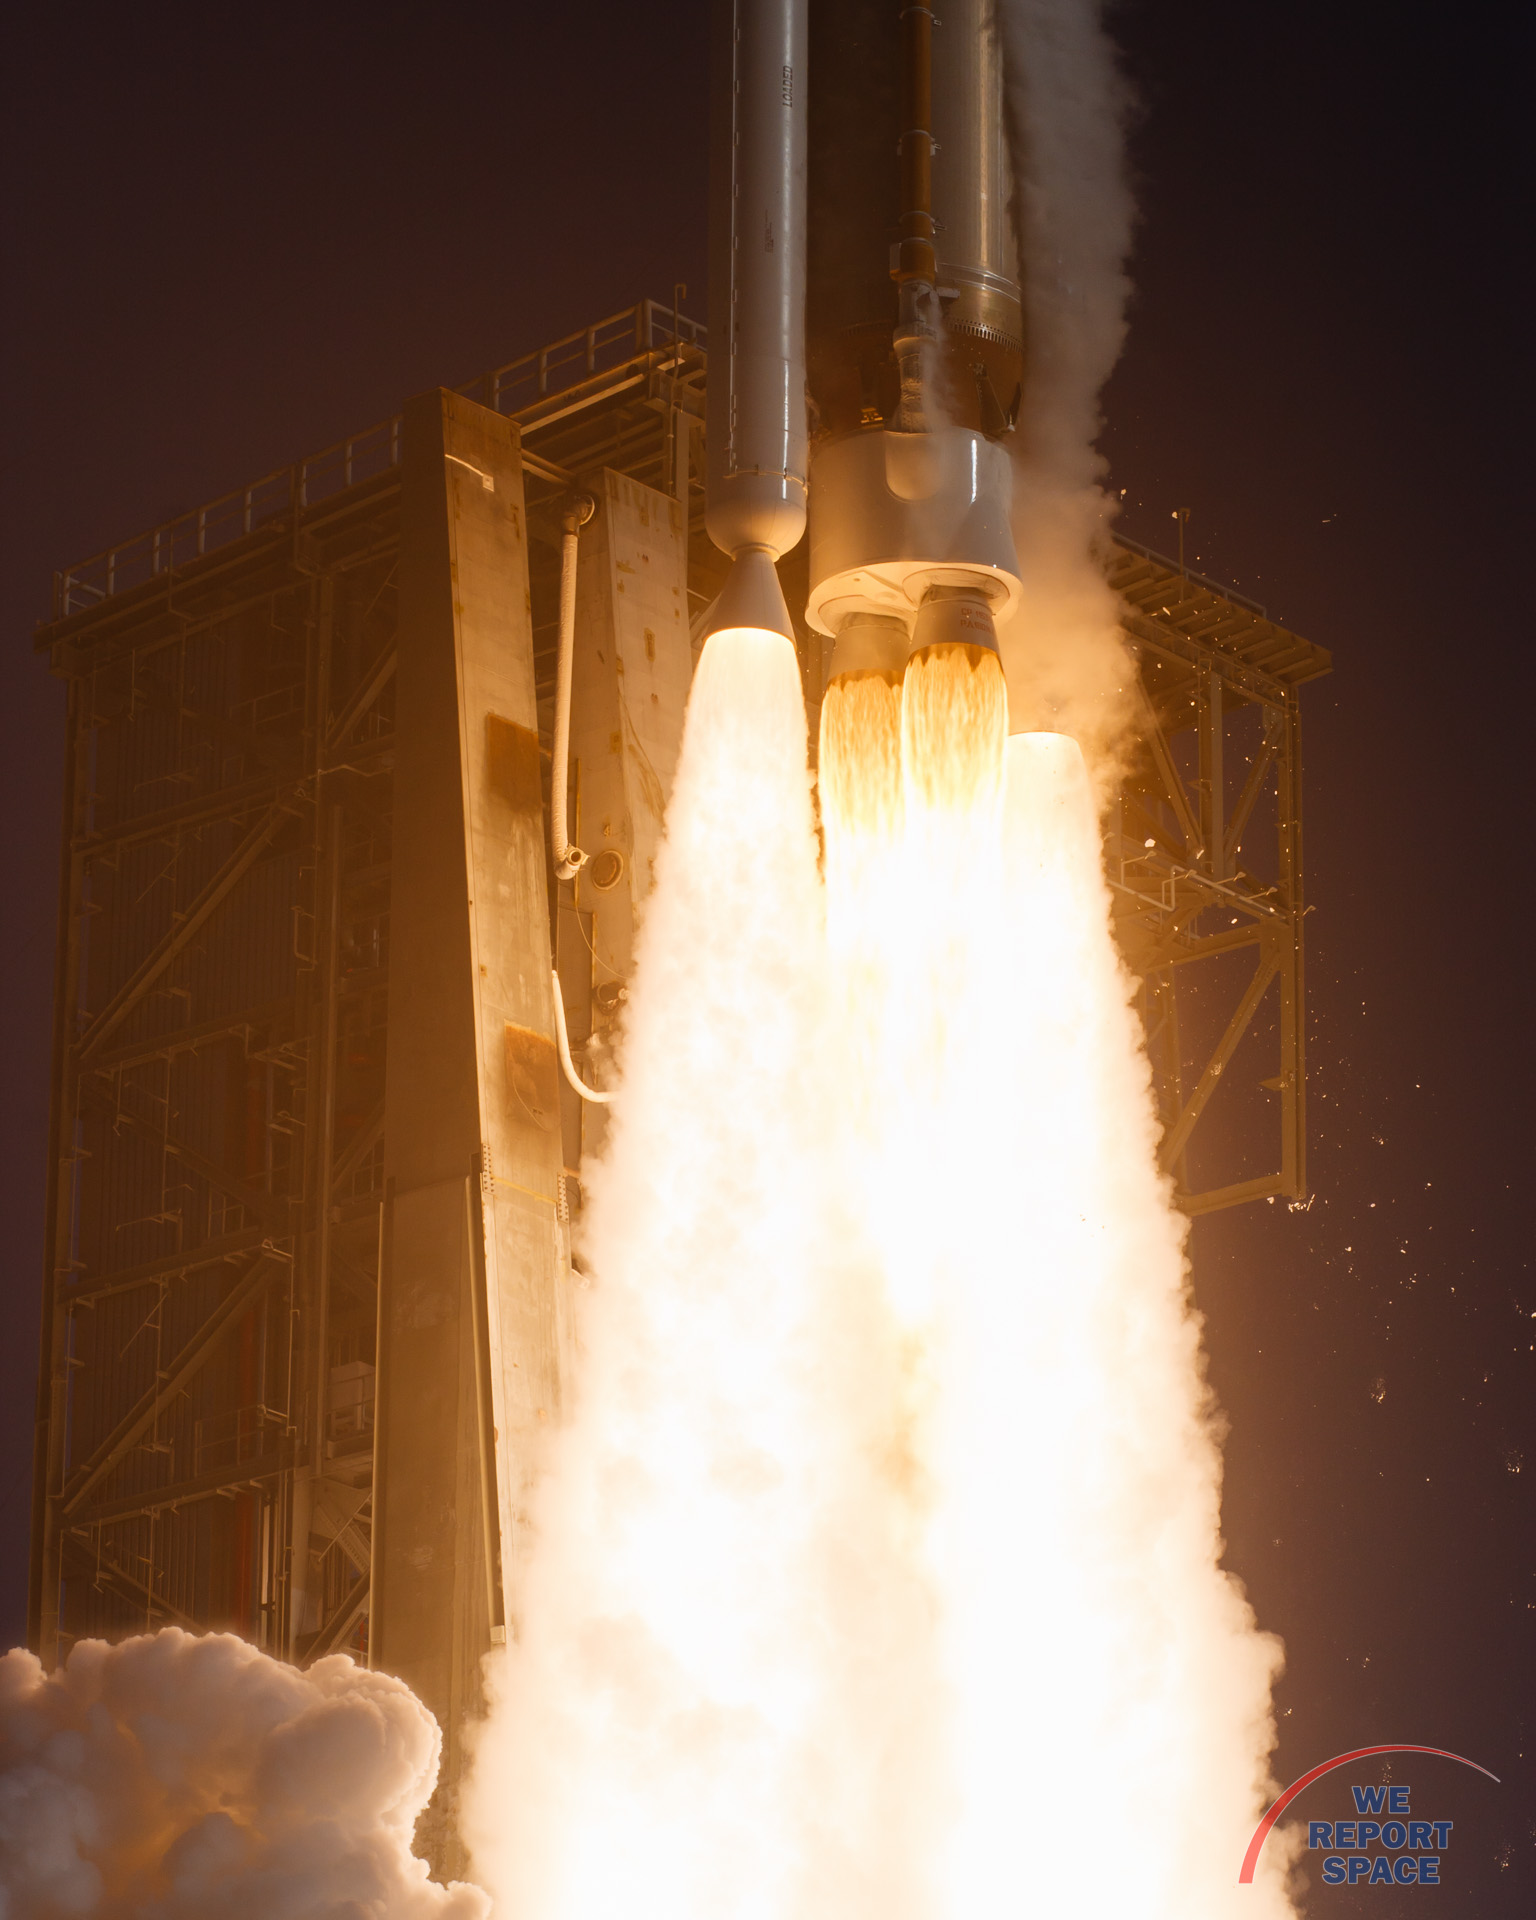
\includegraphics[width=1.in]{figures/8y0ObUW.jpg}}\tiny{$^2$} %https://external-preview.redd.it/raUdEwh8-J01prs80mqdLGG-sVTfg-80YXxwnfwVRtY.jpg?s=eabf5472b6d7a49b7a66ebfecade4f2b9d49dc2f
 \end{columns}
 ~\\
 \pause
 \boxed{\textbf{$\rightarrow$ Prozesse auf mikroskopischer Skala verstehen!}}\\
\end{frame}

\section[]{Einleitung}
\begin{frame}[plain]
% \addtocounter{framenumber}{0}
\frametitle{Inhalt}
\begin{itemize}
 \item \textbf{Methodik}
 \item \textbf{H$_2$O@$\upalpha$-Al$_2$O$_3$(0001)}: Stabilität, Vibrationsfrequenzen und Reaktivität
 \item \textbf{H$_2$O@$\upalpha$-Al$_2$O$_3$(0001)}: Simulation von Molekularstrahlexperimenten mit AIMD
 \item \textbf{H$_2$O@$\upalpha$-Al$_2$O$_3$(11\=20)}: Stabilität und Vibrationsfrequenzen
% \item \textbf{Zusammenfassung und Ausblick}
 \end{itemize}
\end{frame}


\begin{frame}
% \addtocounter{framenumber}{1}
 \frametitle{Aufbau und Eigenschaften von $\upalpha$-Al$_2$O$_3$}
 \begin{columns}
  \column{.5\textwidth}
  \begin{figure}
  \centering
  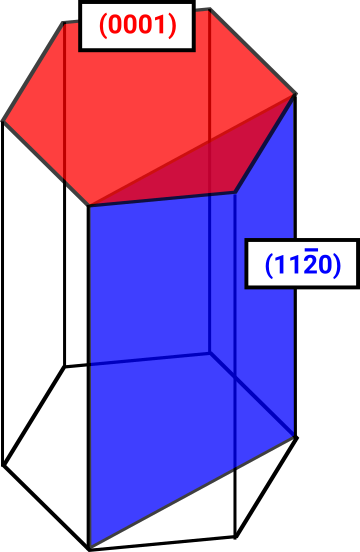
\includegraphics[width=0.3\textwidth]{figures/al2o3-crystal.png}
  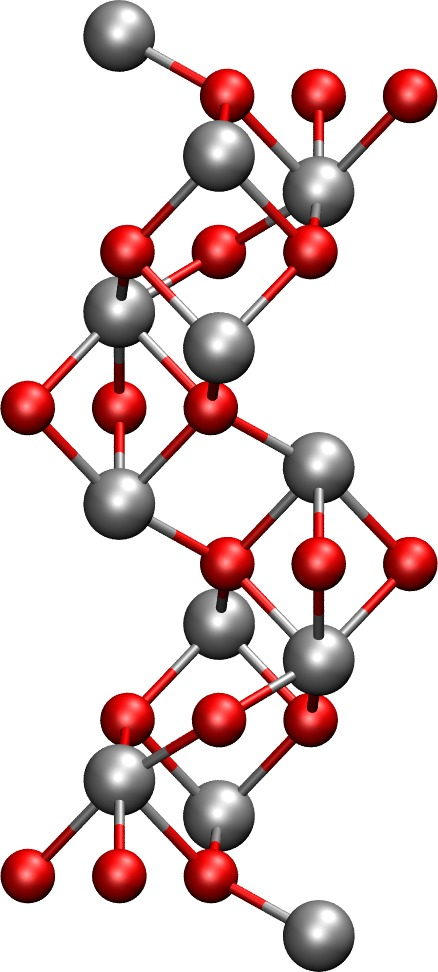
\includegraphics[width=0.2\textwidth]{figures/bulk_UC.jpg}
  \caption{Schema und Einheitszelle}
  \end{figure}
  \column{.5\textwidth}
  \begin{itemize}
  \item hexagonale Zelle
  \item ($2\times 2$) Superzelle
  \item Mohshärte von 9-9,5
  \item Isolator
 % \item Passiviert
 % \item Weißer Feststoff, Verfärbung durch Unreinheiten
 % \item Im UHV (0001) stabiler als (11\=20)
  \end{itemize}
 \end{columns}
 \pause
 \vspace{-.3cm}
\begin{columns}
  \column{.5\textwidth}
  \begin{figure}
  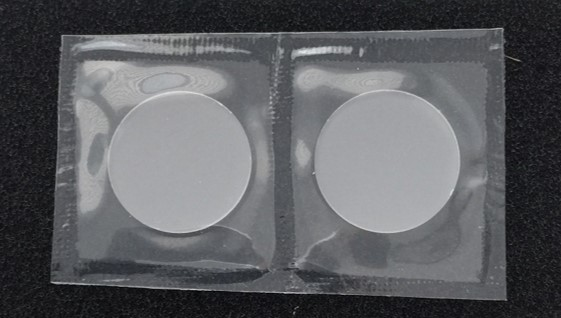
\includegraphics[width=0.7\textwidth]{figures/Al2O3.jpg}
  \caption{Al$_2$O$_3$-Probe (FHI Berlin)}
 \end{figure}
  \column{.5\textwidth}
   \begin{figure}
  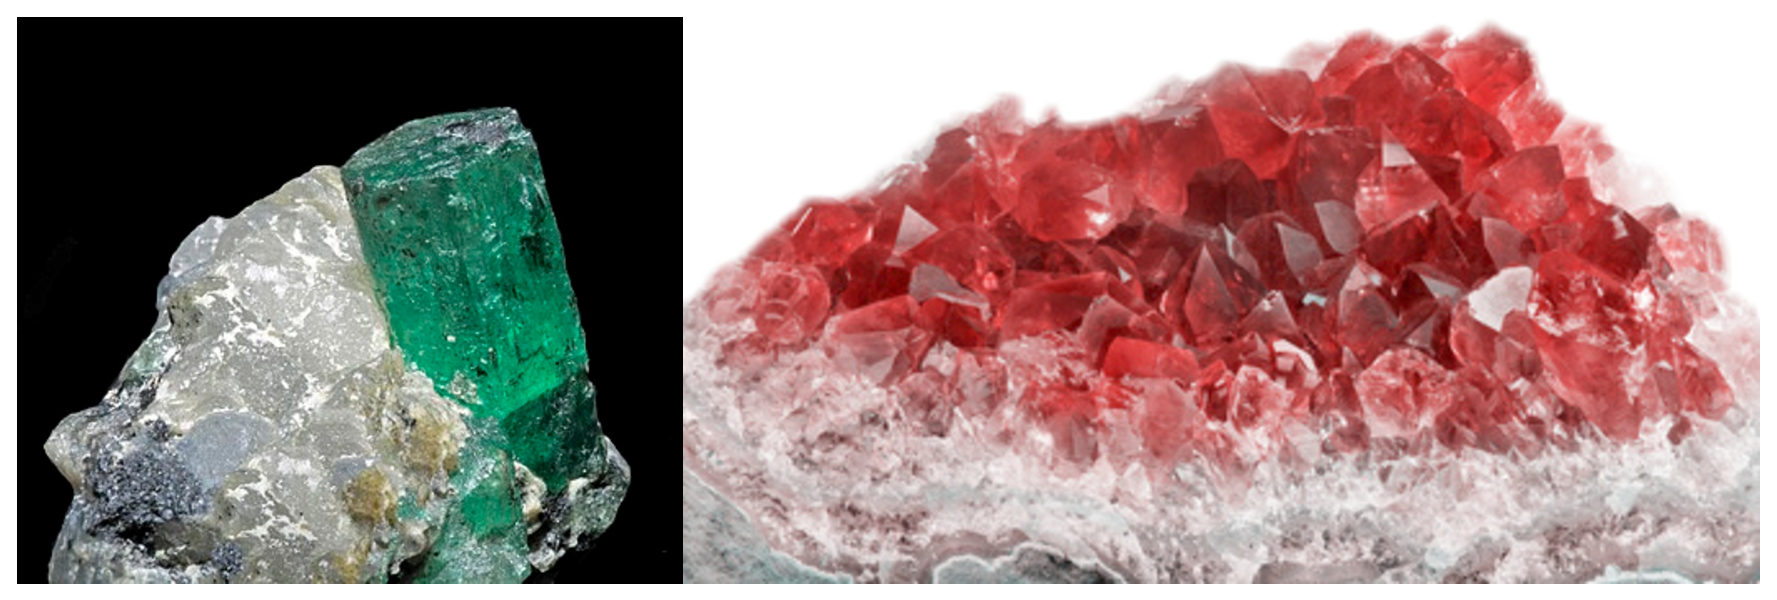
\includegraphics[width=0.9\textwidth]{figures/emerald-ruby.eps}
  \caption{Smaragd (Cr/V); Rubin (Cr)\blfootnote{\tiny{https://goo.gl/images/ZXweQe, https://goo.gl/images/rcqUkB}}}
  \end{figure}
 \end{columns}
\end{frame}

%\begin{frame}
% \frametitle{Methodik}
% \begin{itemize}
%  \item Elektronenstrukturrechnungen (KS-DFT, HF, LMP2)
%  \begin{equation*}
%    \left(-\frac{1}{2}\vec{\nabla}^2_1 + v_{ext}(\vec{r}_1) + v_{H}(\vec{r}_1) + v_{xc}(\vec{r}_1) \right)\psi^{KS}_i(\vec{r}_1) = \varepsilon_i^{KS}\psi^{KS}_i(\vec{r}_1)
%  \end{equation*}
%  \pause
%  \item Vibrationsfrequenzen (harmonische Näherung)
%  \begin{equation*}
%    \textbf{H} \vec{A}_i=\lambda_i\vec{A}_i; ~~~  \omega_i=\sqrt{\lambda_i}
%  \end{equation*}
%  \pause
%  \item \textit{Ab-initio} Molekulardynamik
%    \begin{equation*}
%      -\vec{\nabla}_A V(\{\vec{R}_i\})=M_A\frac{d^2 \vec{R}_A(t)}{dt^2}
%    \end{equation*}
% \end{itemize}
%\end{frame}

\begin{frame}
 \frametitle{Methodik}
 \begin{itemize}
  \item Periodische \textit{slab}-Rechnungen
  \item $\vec{k}$-Raum
  \item Dichtefunktionaltheorie (DFT) vs. Wellenfunktionstheorie (HF, LMP2)
  \item Basis: ebene Wellen (PW) vs. atomzentrierte Orbitale (AO)
  \item Funktionale PBE und B3LYP
  \item Dispersionskorrekturen (D2/D3)
 \end{itemize}

 \centering
 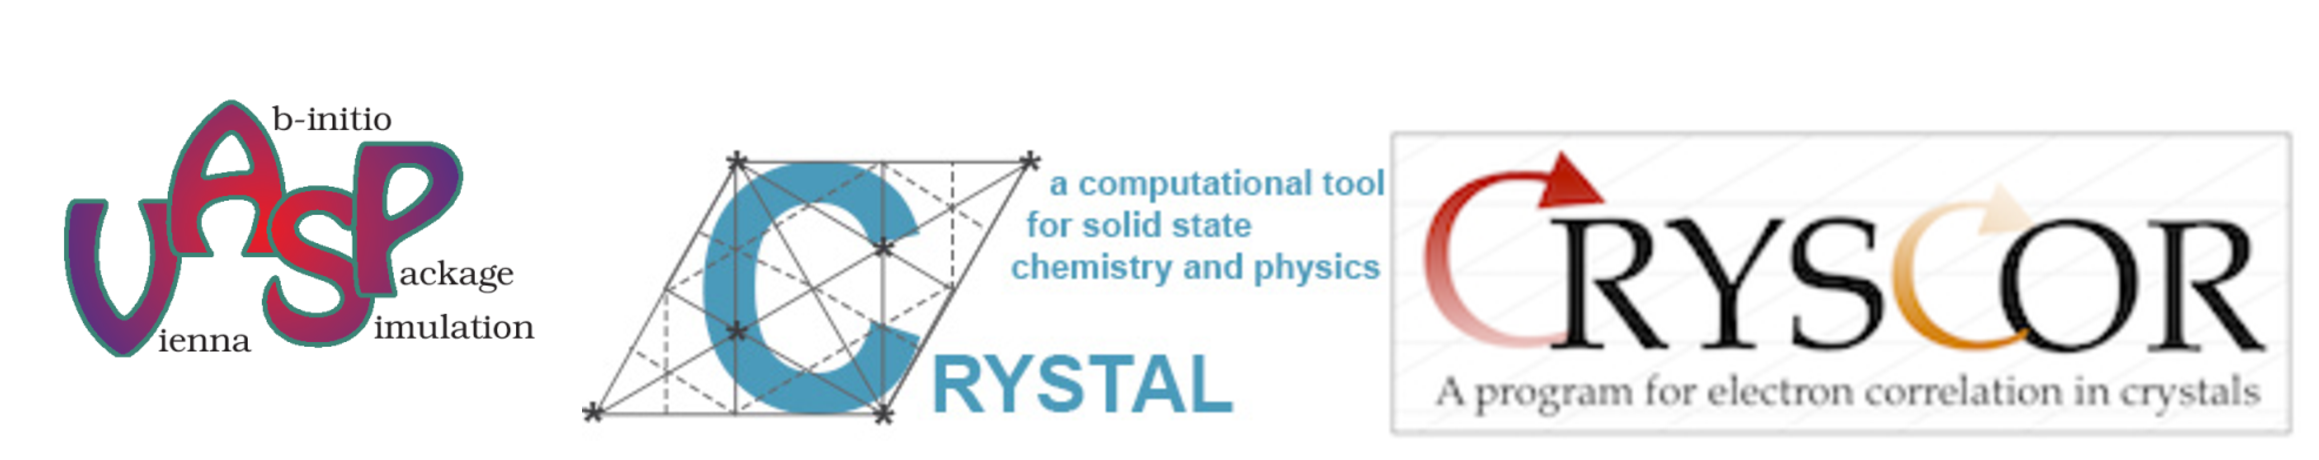
\includegraphics[width=0.7\textwidth]{figures/programs-logos.eps}
\end{frame}

\begin{frame}
\frametitle{Methodik: Eigenschaften}
\begin{itemize}
\item Geometrien
\item Adsorptionsenergien
\item Vibrationsfrequenzen
\item Barrierenhöhen mit Nudged Elastic Band (NEB)
\end{itemize}
\end{frame}

\section{H$_2$O@Al$_2$O$_3$(0001): Stabilität, Schwingungen und Reaktivität}
\begin{frame}
 \frametitle{Modell der $\upalpha$-Al$_2$O$_3$(0001) Oberfläche}
 \begin{columns}
  \column{0.5\textwidth}
   \begin{figure}
  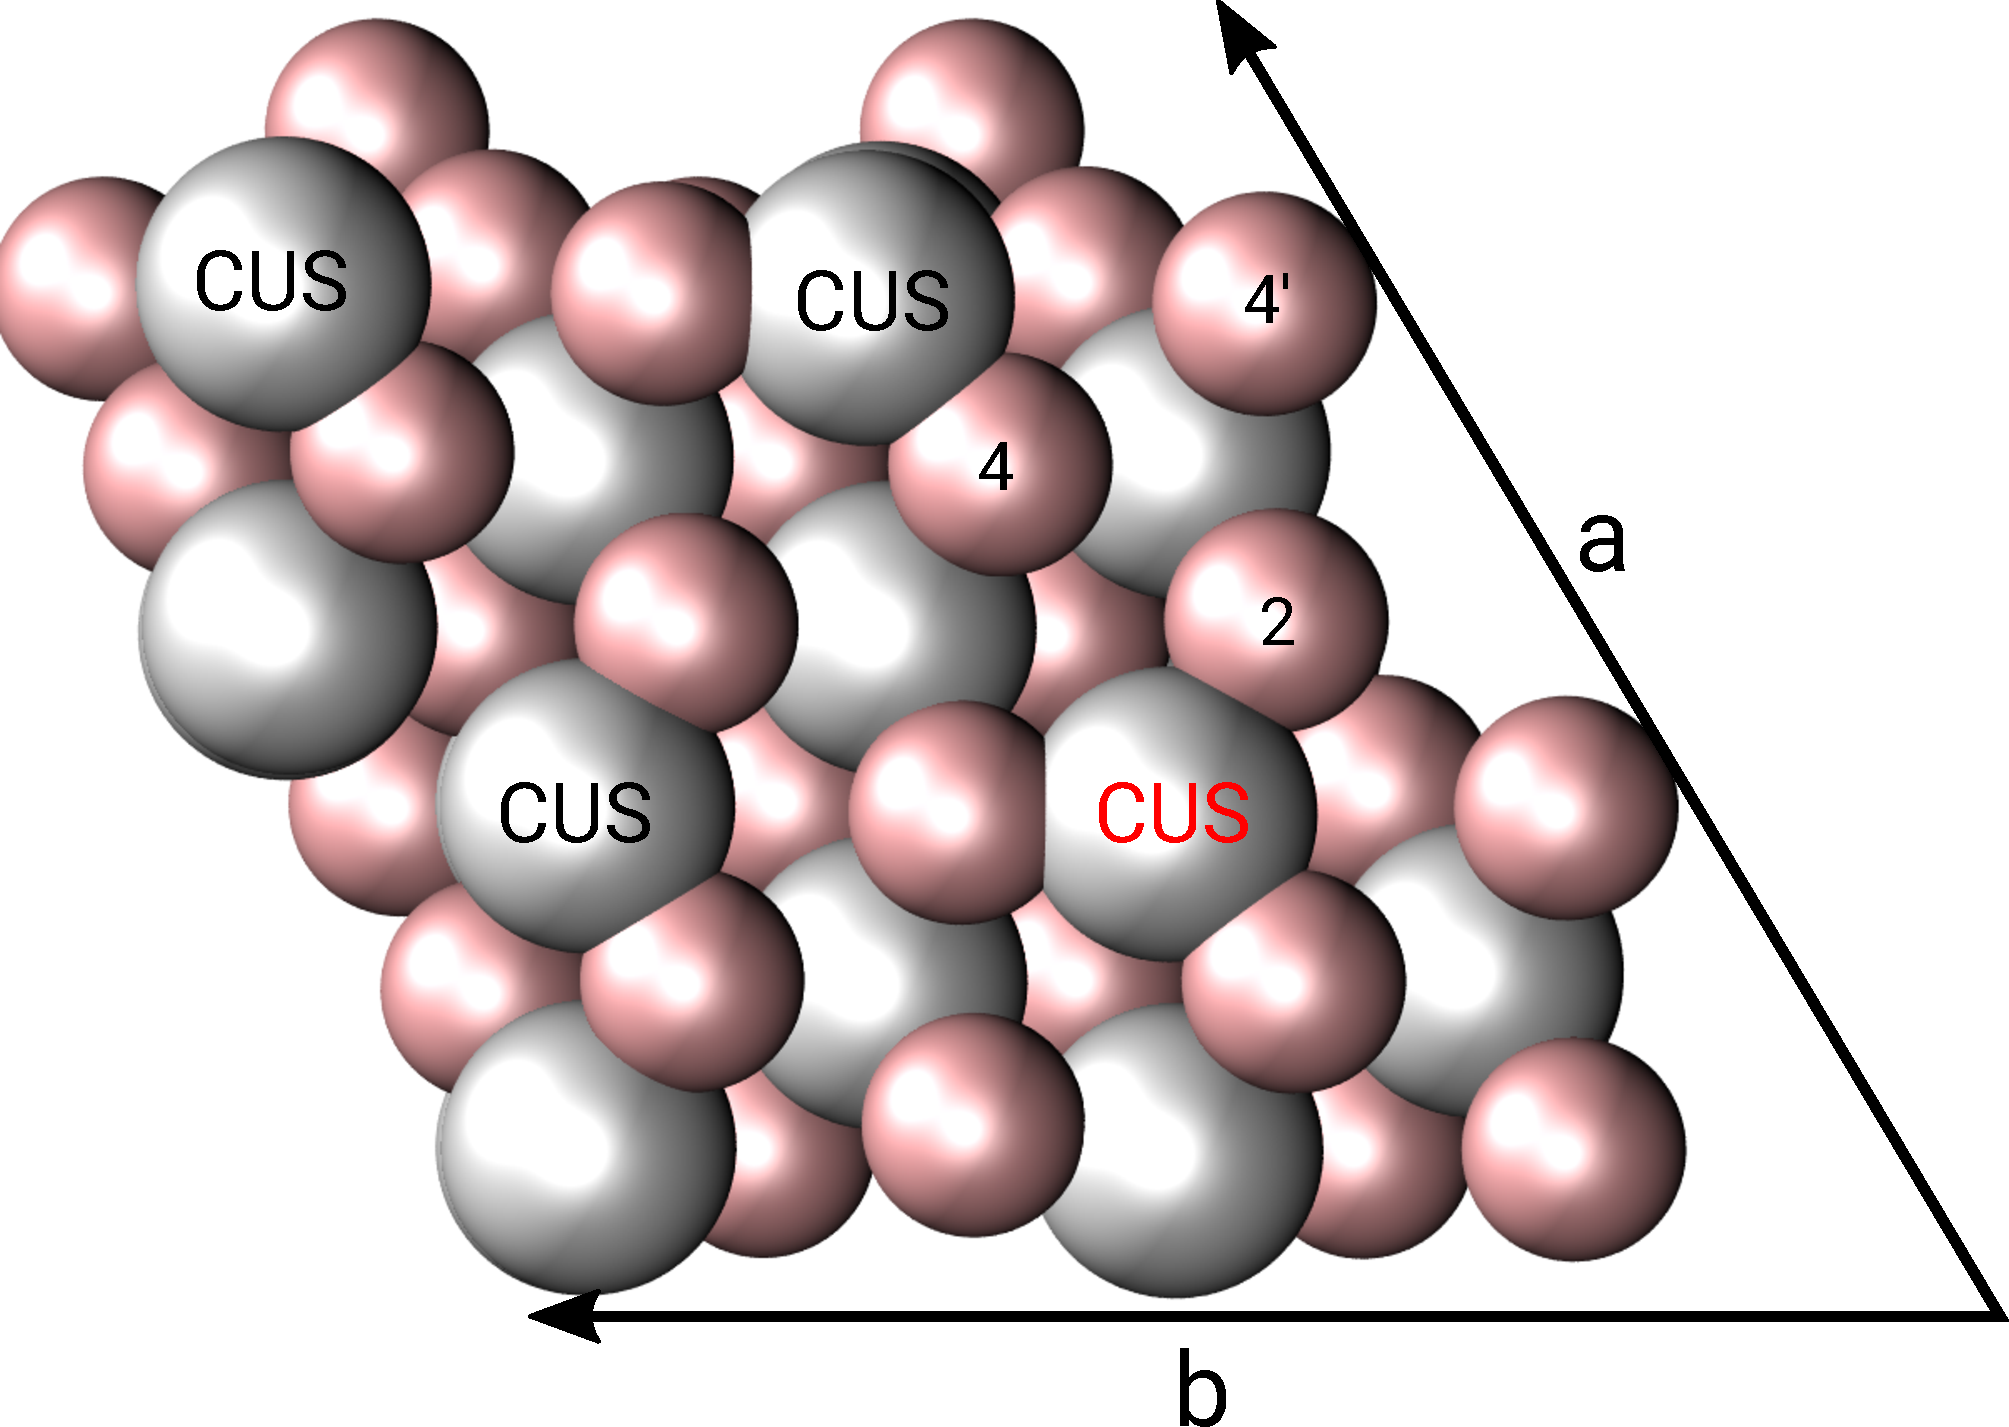
\includegraphics[width=0.9\textwidth]{figures/surf_0K_axes.pdf}
  \caption{Draufsicht, Al grau, O rosa. \textbf{C}oordinatively \textbf{U}nsaturated \textbf{S}ite}
  \end{figure}
  \column{0.5\textwidth}
  \begin{figure}
  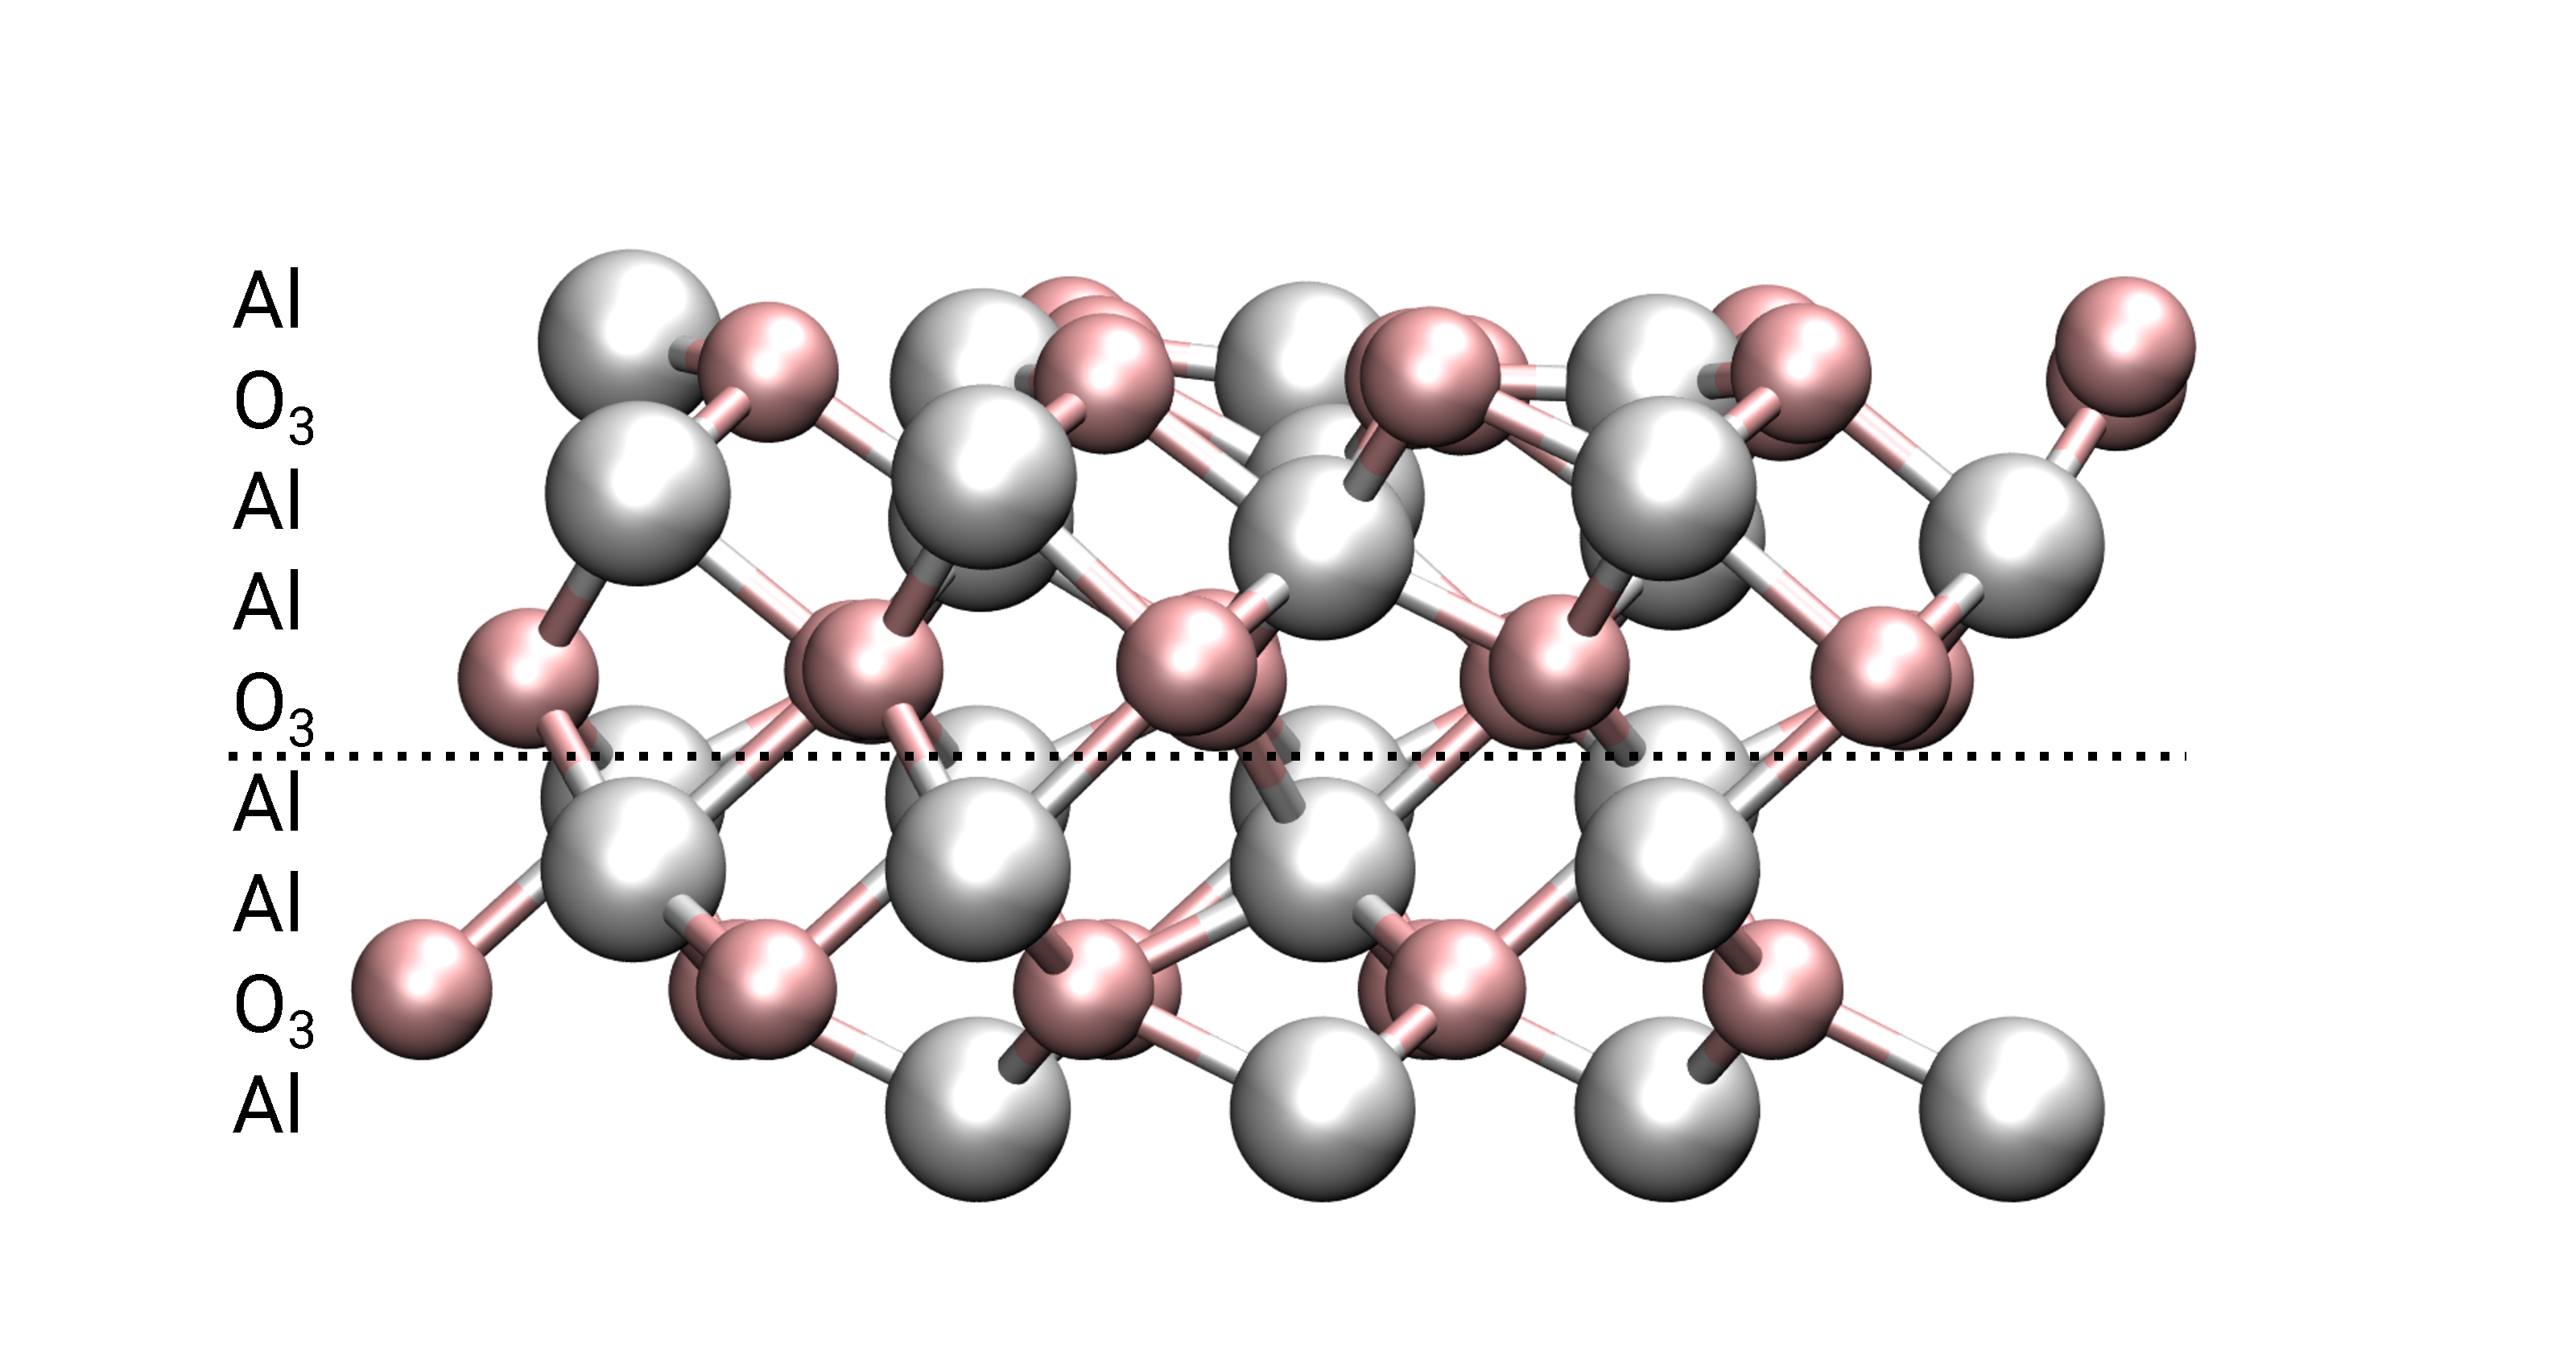
\includegraphics[width=1.\textwidth]{figures/surf_0K-side.pdf}
  \caption{Seitenansicht, Sequenz Al-O$_3$-Al...}
  \end{figure}
  \end{columns}
 \hrule
 \begin{itemize}
  \item Optimierte Struktur (UHV $0\,$K)
  \item Al terminierte Oberfläche
  \item 4 CUS Al Atome, 12 dreifach-koordinierte O Atome
  \item ($2\times 2$) Superzelle
 \end{itemize}
\end{frame}

\begin{frame}
 \frametitle{H$_2$O-Adsorption}
 \begin{itemize}
 \item Stabilste adsorbierte Spezies, 1/4 Bedeckung
\end{itemize}
\vspace{-.2cm}
 \begin{figure}
  \centering
  \subfigure[mol]{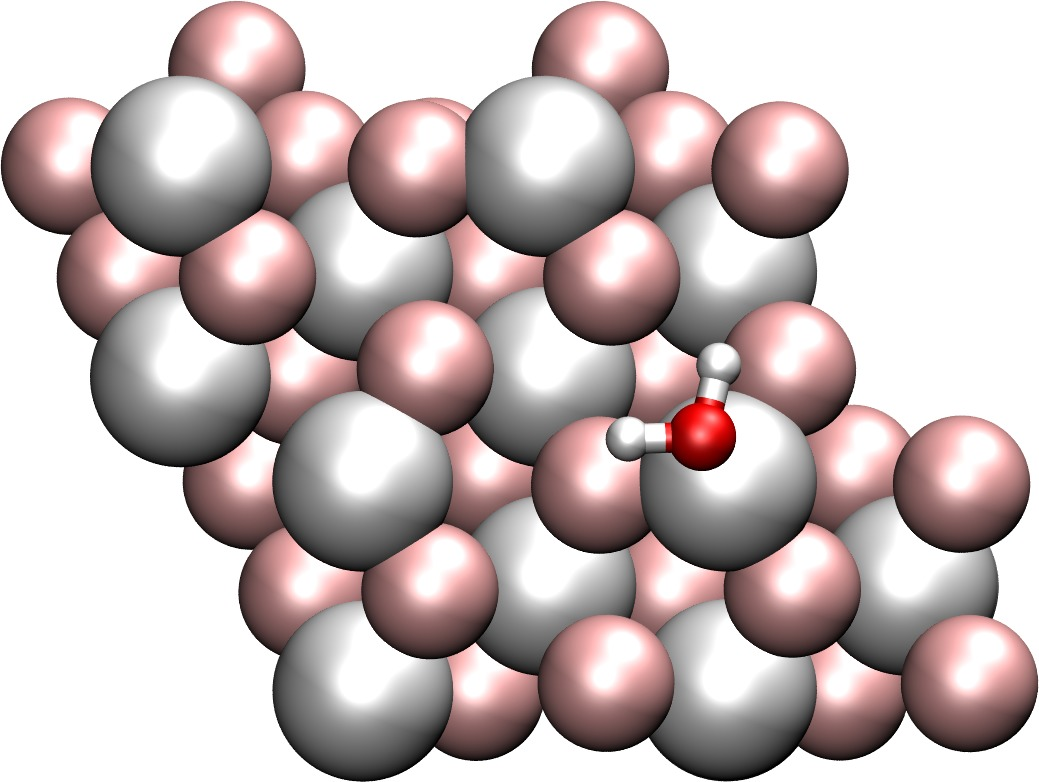
\includegraphics[width=0.35\textwidth]{figures/0001_mol_top.jpg}}
  \subfigure[1-2]{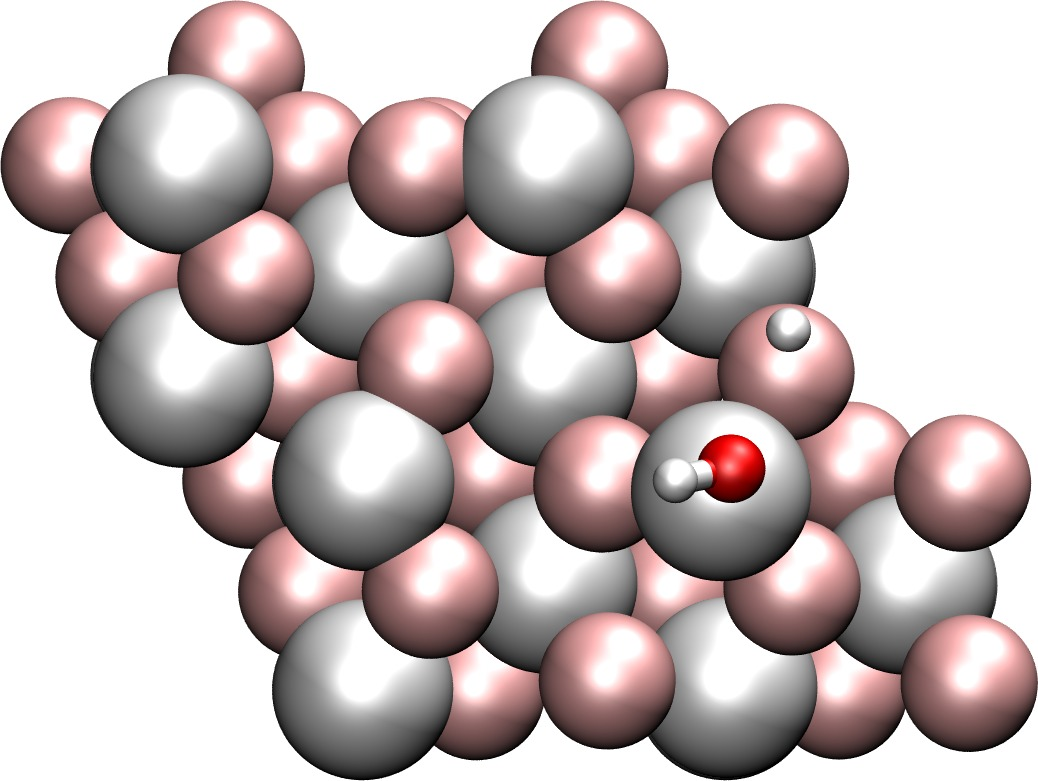
\includegraphics[width=0.35\textwidth]{figures/0001_1-2-diss_top.jpg}}
  \subfigure[1-4]{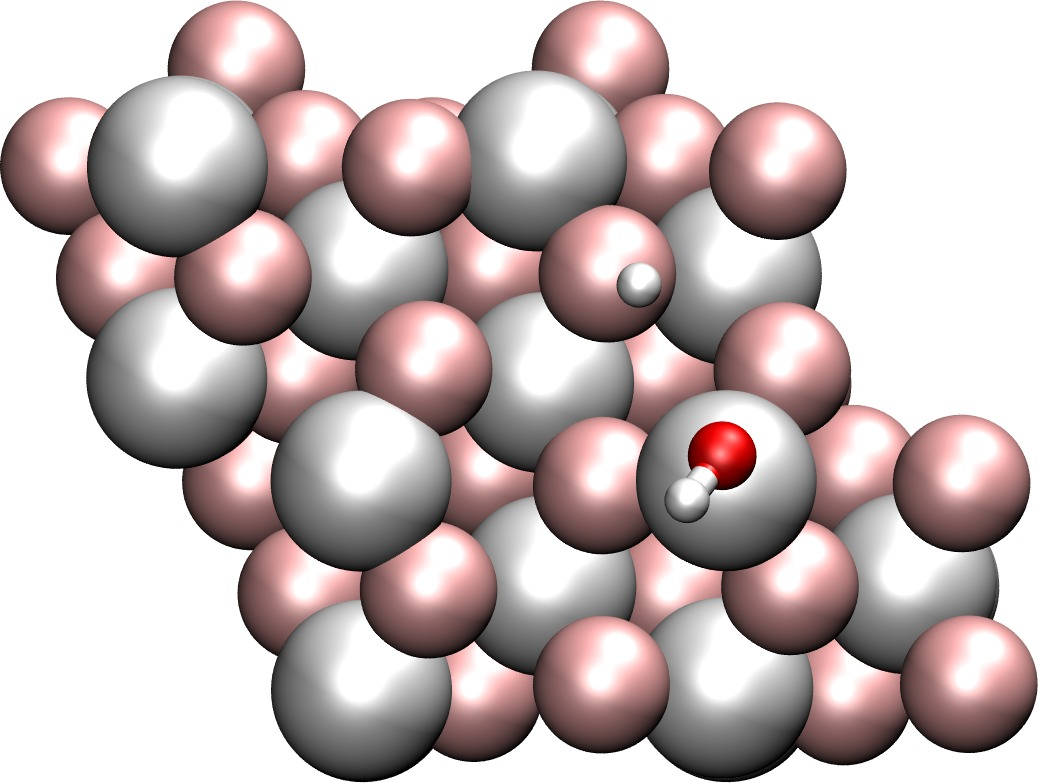
\includegraphics[width=0.35\textwidth]{figures/0001_1-4-diss_top.jpg}}
  \subfigure[1-4$^\prime$]{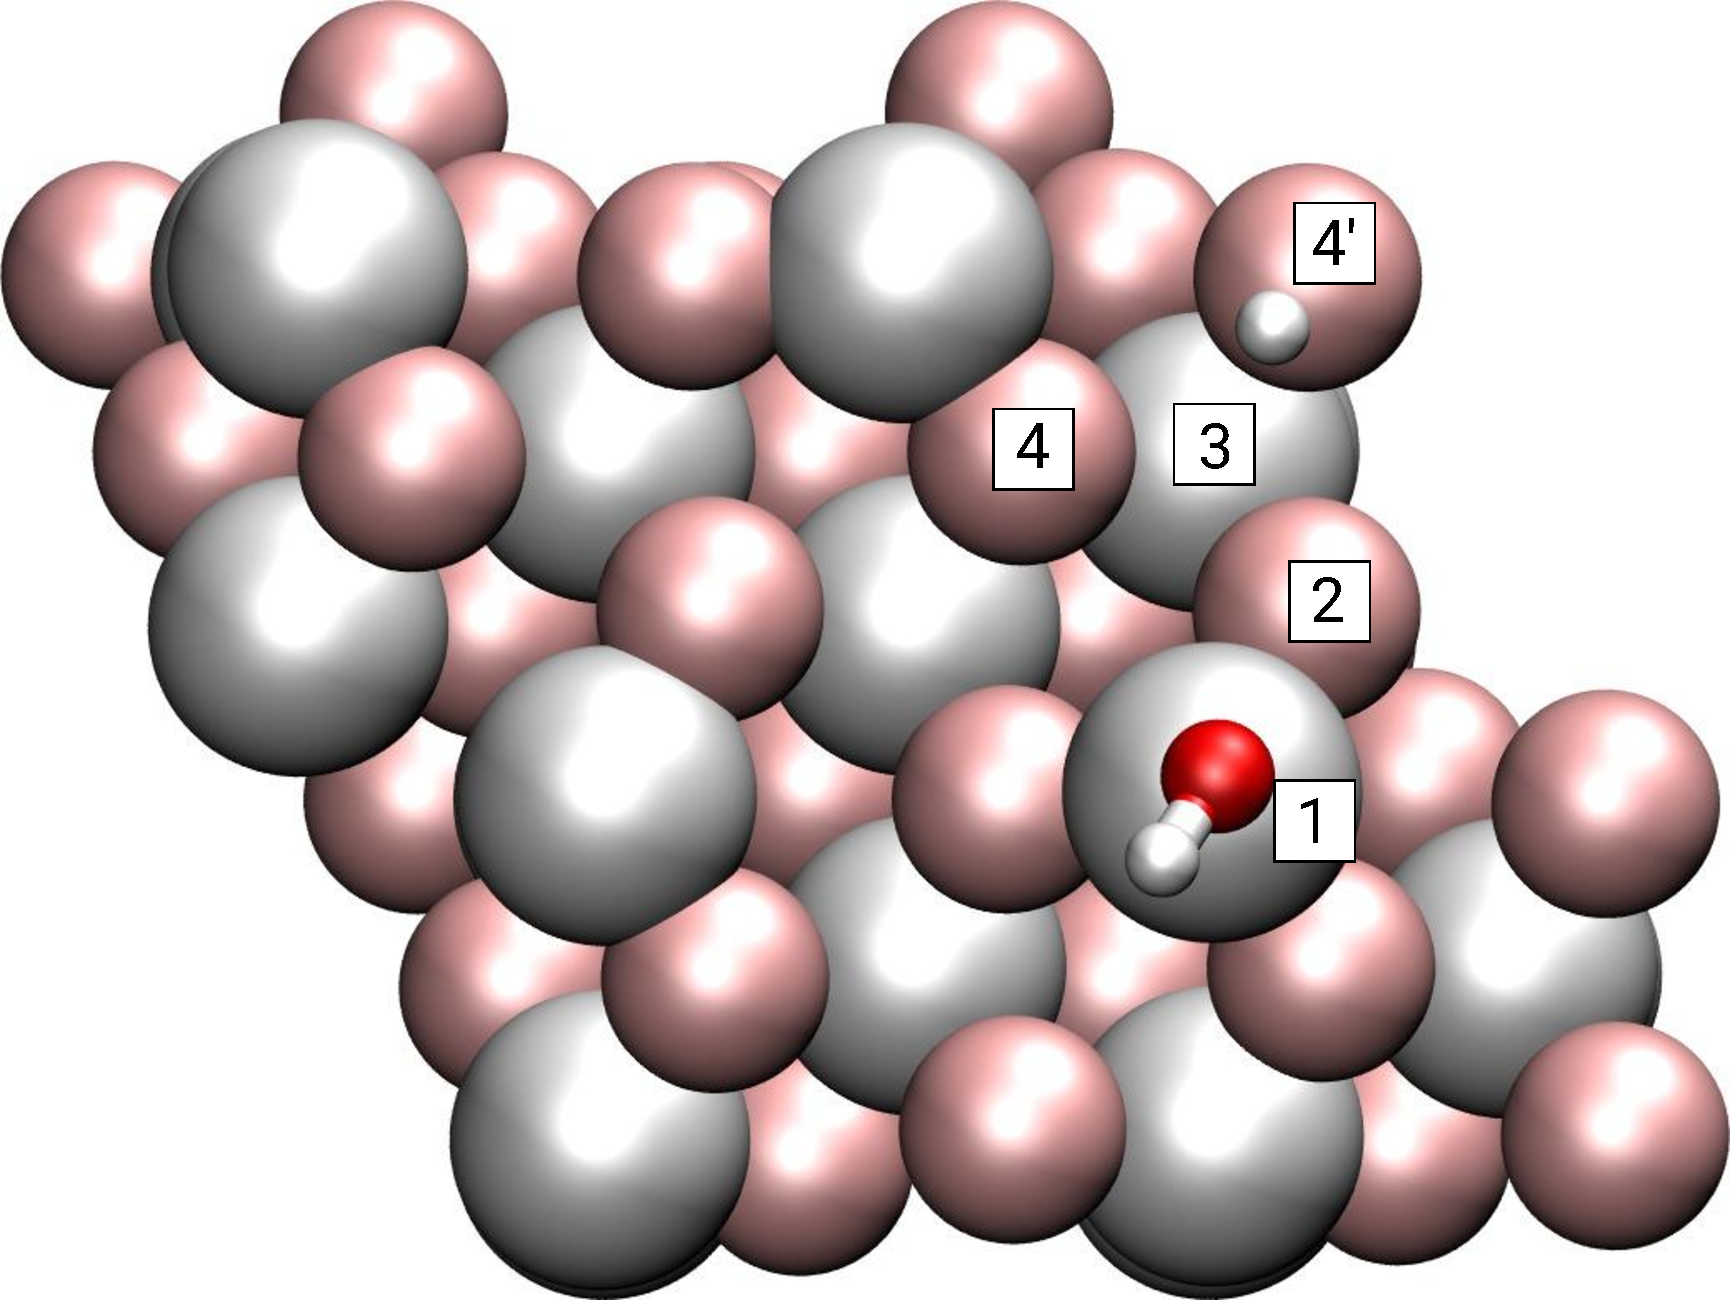
\includegraphics[width=0.35\textwidth]{figures/0001_1-4p-diss_top_label.pdf}}
 \end{figure}
% \pause
% \item Schwingungsfrequenzen für Vergleich mit SFG Spektroskopie
% \pause
% \item Diffusionsreaktion Df-H-4-2
% \begin{figure}
%  \centering
%  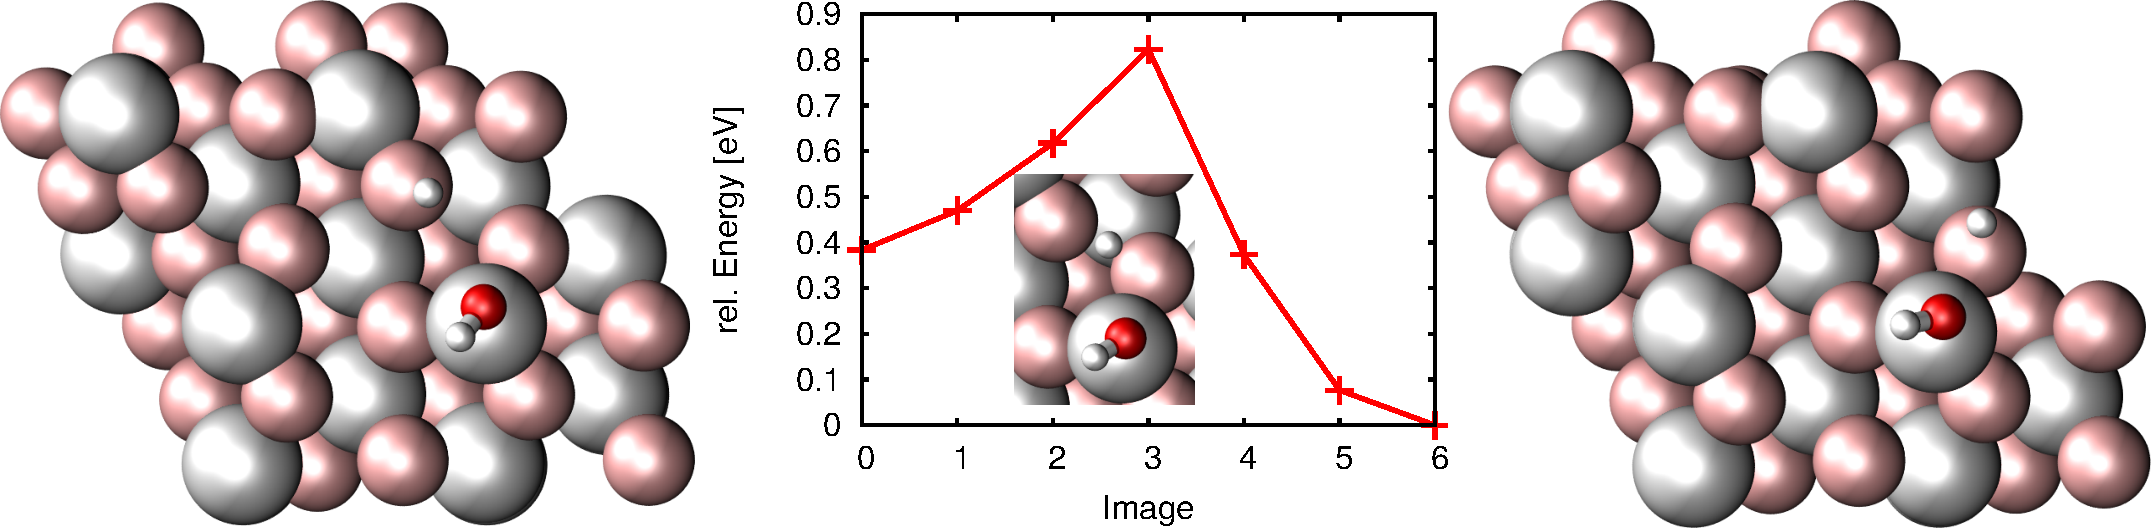
\includegraphics[width=.7\textwidth]{figures/df-h-4-2.pdf}
%  \caption{Wasserstoffdiffusion von 1-4 nach 1-2, NEB Pfad mit Übergangszustand}
% \end{figure}
% \end{itemize}
 \end{frame}

\begin{frame}
 \frametitle{Adsorptionsenergien}
 \begin{table}[!h]
  \centering
   \caption{Adsorptionsenergien $E_\textrm{ads}$ in eV.} %der molekularen und der zwei dissoziierten adsorbierten Spezies von H$_2$O auf der Al$_2$O$_3$(0001) Oberfläche, Vergleich von plane wave Basis (PW) und Atomorbitalbasis (AO).
   %$E_{\textrm{ads}}=E_{\textrm{ads. Spezies}}-(E_{\textrm{freies Wassermolekül}}+E_{\textrm{Oberfläche}})$}
  \begin{tabular}{ll|cc}
  \toprule
Basis& Methode & mol &1-4 diss\\\midrule
  \multirow{3}{1cm}{PW}&PW91$^1$\blfootnote{$^1$\textit{J. Phys. Chem. C} \textbf{116}, 26829 (2012)} &\textbf{-1.25} &\textbf{-1.25} \\
  &PW91+D2$^1$&-1.40 &\textbf{-1.45} \\\hline
  &PBE+D2 & \textbf{-1.31} & -1.21 \\
  %&PBE+D3 &-1.29&-1.63 &-1.30 \\
  \midrule \pause
  \multirow{4}{1cm}{AO}&PBE+D3 &\textbf{-1.41} &-1.32 \\
  &B3LYP+D3 &\textbf{-1.43} &-1.40 \\
  &HF &-1.14 &\textbf{-1.19} \\
  &LMP2 &\textbf{-1.34} &-1.26\\
  %&LMP2 (basis 9) &-1.31 &-1.61 &-1.18 \\
  \bottomrule
  \end{tabular}
 \end{table}
\end{frame}

\begin{frame}
 \frametitle{Vibrationsfrequenzen der Dissoziierten Wasserspezies}
% \begin{columns}
% \column{0.4\textwidth}
  \centering
  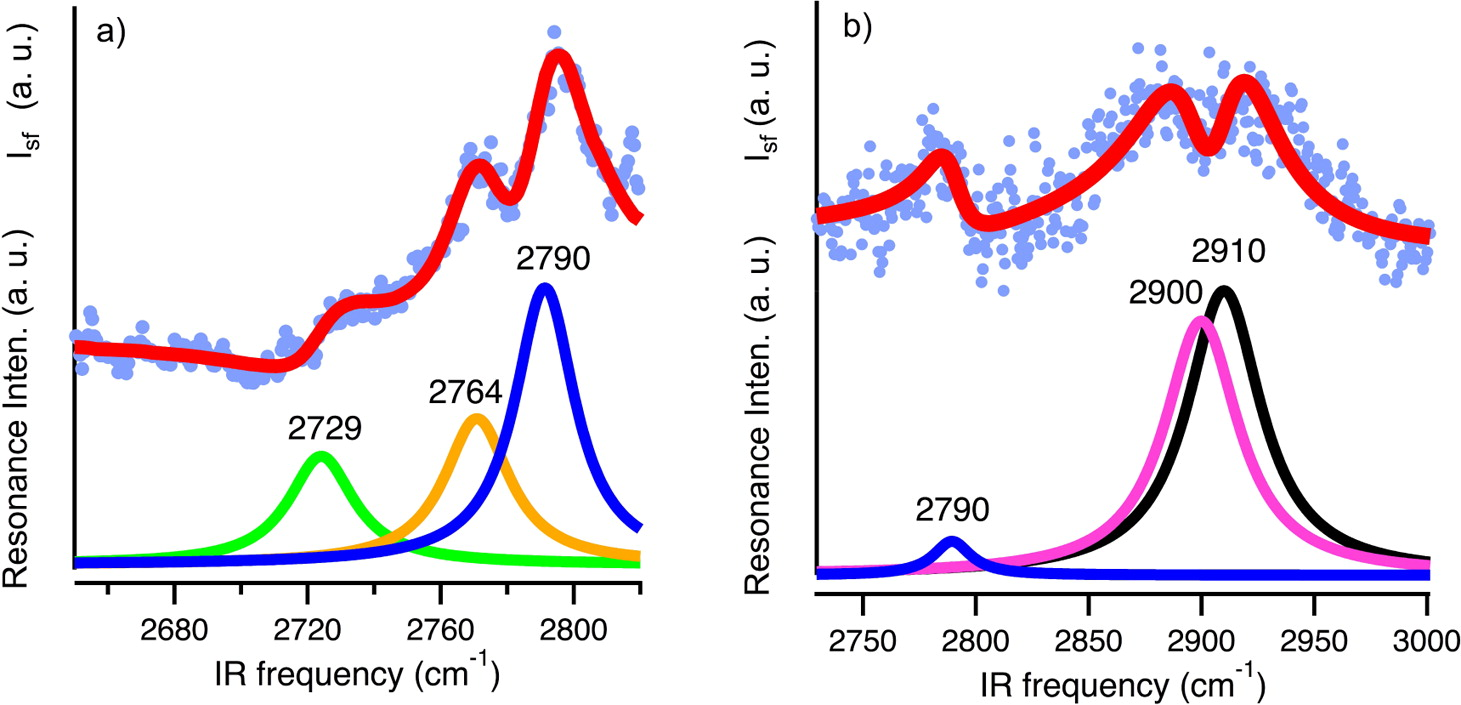
\includegraphics[width=.7\textwidth]{figures/0001_OD_vib_exp.jpeg}\\
  \footnotesize{J. Phys. Chem. C \textbf{2014}, \textit{118}, 13623--13630.}
% \column{0.6\textwidth}
  \begin{table}[!h]
  \centering
  \caption{$\tilde{\nu}$ in cm$^{-1}$, gerechnet für deuteriertes Wasser.}
  \begin{tabular}{l|cc}
  \toprule
 Streckschw. &B3LYP+D3/AO & Exp.\\\midrule
 1-2 OD$_{surf}$&2697&2729\\
 1-4 OD$_{surf}$&2715&2764\\
%  1-4$^\prime$ OD$_{surf}$&2583&2790\\
 1-4 OD$_{ads}$&2873&2900\\
%  1-4$^\prime$ OD$_{ads}$&2697&2900\\
 1-2 OD$_{ads}$&2883&2910\\\bottomrule
  \end{tabular}
 \end{table}
 %\end{columns}
 \end{frame}
 \begin{frame}
 \frametitle{Relative Vibrationsfrequenzen}
  \begin{table}[!h]
  \centering
    \caption{$\Delta \tilde{\nu}$ der dissoziierten Wasserspezies in cm$^{-1}$.}
    \vspace{-0.5cm}
  \begin{tabular}{c|cc|c|c}
  \toprule
& \multicolumn{2}{c}{AO} & PW & \\
 Streckschw. &PBE+D3 & B3LYP+D3 & PBE+D2 & Exp.\\\midrule
 1-2 OD$_{\textrm{ads}}-$1-2 OD$_{surf}$& 212& 186& 181& 191 \\
 1-2 OD$_{\textrm{ads}}-$1-2 OD$_{ads}$ & 187& 168& 163& 146\\
 1-2 OD$_{\textrm{ads}}-$1-4 OD$_{surf}$& 13& 10& 15& 10\\\bottomrule
  \end{tabular}
 \end{table}
\end{frame} 

\begin{frame}
 \frametitle{Aktivierungsbarrieren mit Hybridfunktionalen und LMP2}
 \begin{itemize}
  \item GGA Funktionale (hier PBE) unterschätzen Aktivierungsbarrieren $\rightarrow$ Hybridfunktional, Störungstheorie
 \end{itemize}
 \centering
   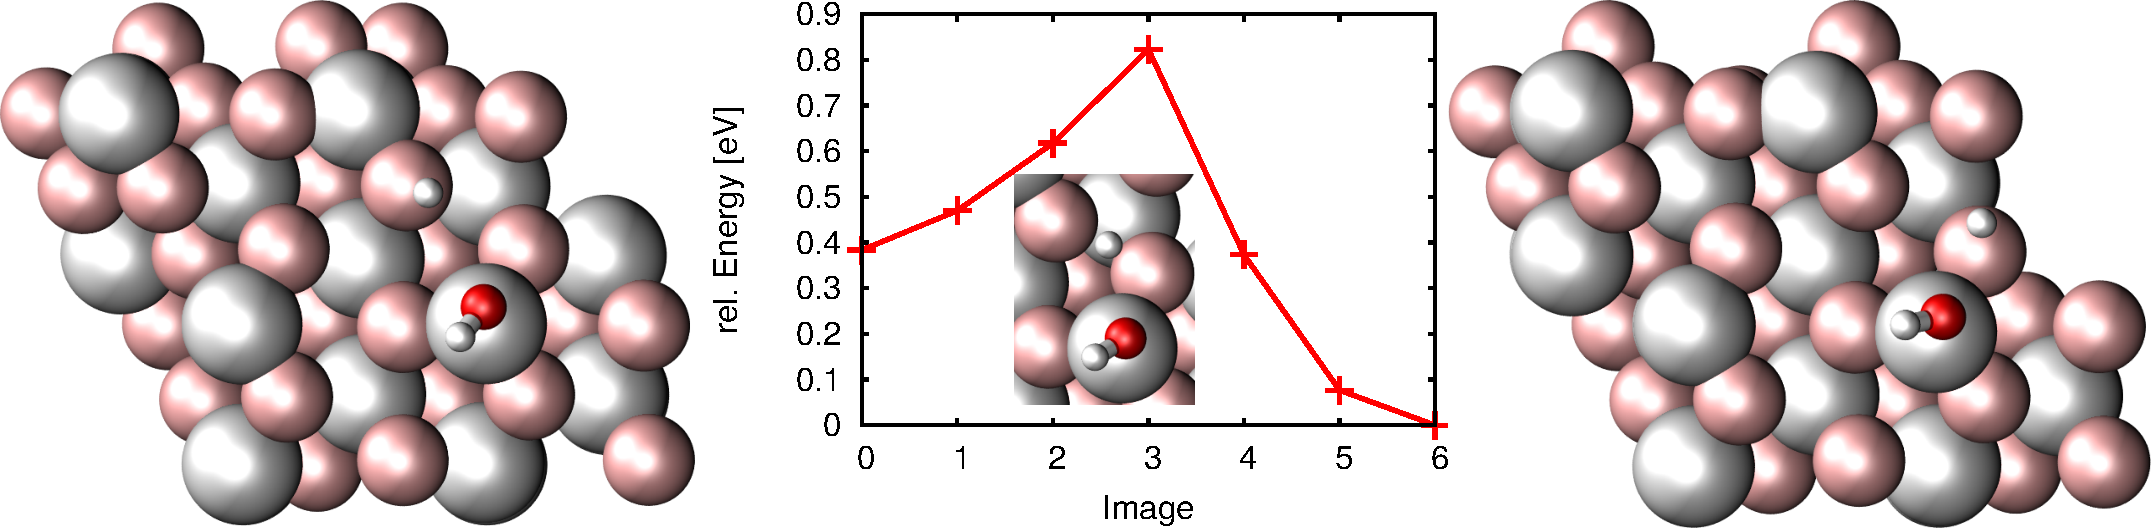
\includegraphics[width=.75\textwidth]{figures/df-h-4-2.pdf}
     \vspace{-.2cm}
     \pause
\begin{table}[!h]
  \centering
  \caption{$k(T)=\frac{k_BT}{h}e^{-\Delta G^\ddagger(T)/(k_BT)}$}
  \vspace{-.5cm}
  \begin{tabular}{l|cc|c}%|cc
  \toprule
    Methode& B3LYP+D3/AO&LMP2/AO &PBE+D2/PW\\\midrule
%     basis&AO-8&AO-9&PW\\\midrule
   $\Delta E^\ddagger$ [eV] &0.69 & 0.60&0.44\\
   $\Delta G^\ddagger$(300K) [eV]&0.58 & 0.49$^\ast$ &0.29\\
   $k$(300K) [s$^{-1}$]&$1.2\times 10^3$ & $3.7\times 10^{4\ast}$&$9.1\times 10^7$\\\bottomrule 
  \end{tabular}
\end{table}
$^\ast$ \textit{Beitrag der Schwingungen ist abgeschätzt durch B3LYP+D3.}
 \centering
 \fbox{\parbox{\textwidth}{S. Heiden, D. Usvyat, P. Saalfrank, \textit{J. Phys. Chem. C} \textbf{2019}, \textit{accepted}}}
\end{frame} 

%\begin{frame}
% \frametitle{Erfolge}
% \begin{itemize}
%  \item Rekalkulierung der Adsorptionsenergien mit atomzentrierter Orbitalbasis
%  \item Verbesserte Übereinstimmung der theoretischen Beschreibung der Vibrationsfrequenzen im Bezug auf SFG Experimente
%  \item Verbesserung der Aktivierungsbarriere für eine Diffusionsreaktion
% \end{itemize}
% \newline~\newline~\newline
% \centering
% \fbox{\parbox{\textwidth}{S. Heiden, D. Usvyat, P. Saalfrank, \textit{J. Phys. Chem. C} \textbf{2019}, %\textit{accepted}}}
%\end{frame}

\section{H$_2$O@Al$_2$O$_3$(0001): Simulation von MBS-Experimenten~~~~~~~~~~}
\begin{frame}
 \frametitle{Motivation: (0001) Molekularstrahlexperiment}
Aufbringen von Wasser auf die Oberfläche: 
 \begin{itemize}
 \item MBS (molecular beam source) vs. Pinhole Dosing
 \item UHV, Molekularstrahl auf Oberfläche vs. Wasser mit hohem Druck
 \item Nicht-Gleichgewichtsbedingungen vs. Gleichgewichtssituation
 \item \textbf{Erhöhte Dissoziationswahrscheinlichkeit mit MBS}
 \newline~
 \pause \hrule
 \newline~
 \item Modellieren des Adsorptions-/Dissoziationsprozesses mit \textit{ab initio} Molekulardynamik Simulationen
 \item Verschiedene Oberflächen- und Strahlenmodelle
\end{itemize}
\pause
\newline~\newline~
\fbox{\parbox{0.98\textwidth}{Heiden, S.; Wirth, J.; Campen, R. K.; Saalfrank, P., \textit{J. Phys. Chem. C} \textbf{2018}, \textit{122} (27), 15494--15504.}}
\end{frame}

\begin{frame}
 \frametitle{(0001) Oberflächen- und Strahlenmodelle}
 \begin{columns}
  \column{.5\textwidth}
  Oberflächenmodelle
  \begin{itemize}
   \item Reine Oberfläche bei $0$ und $300\,$K
   \item Präadsorbierte Oberfläche bei $0$ und $300\,$K
  \end{itemize} 
  \centering
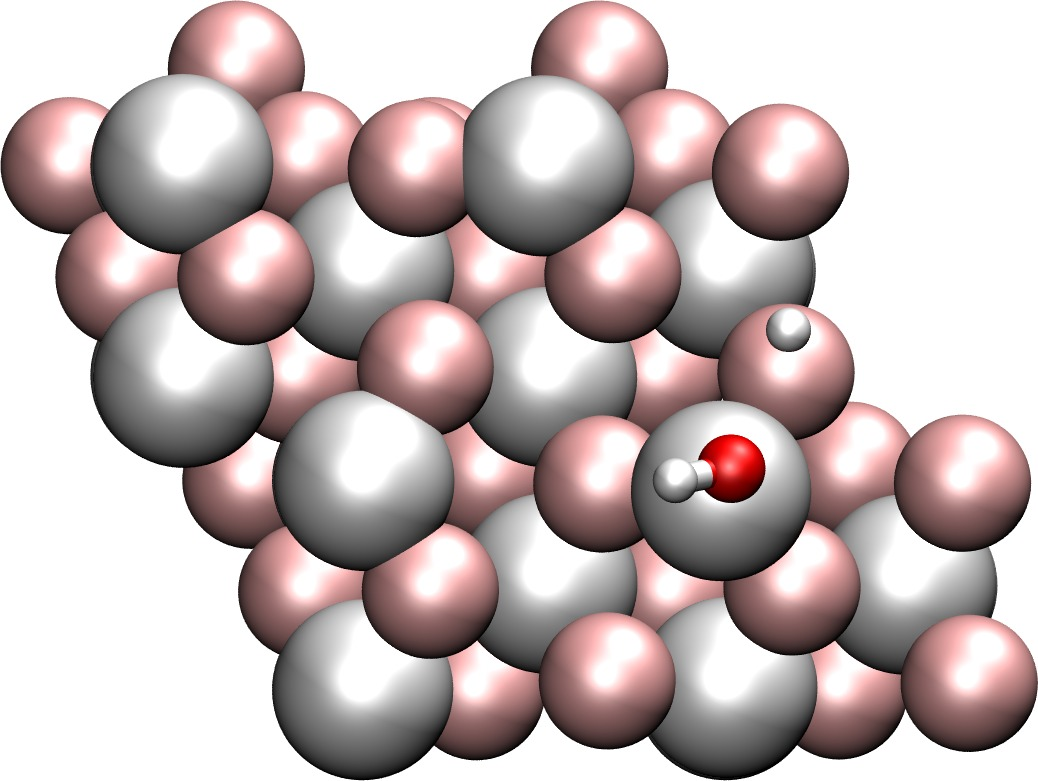
\includegraphics[width=1.\textwidth]{figures/0001_1-2-diss_top.jpg}
\newline
\pause
  \column{.5\textwidth}
  Strahlenmodelle
  \begin{itemize}
   \item starres Wassermolekül
   \item (D$_2$O)$_4$ Cluster
   \item Rotatorisch/Vibratorisch angeregtes Wasser
  \end{itemize}
   \centering
 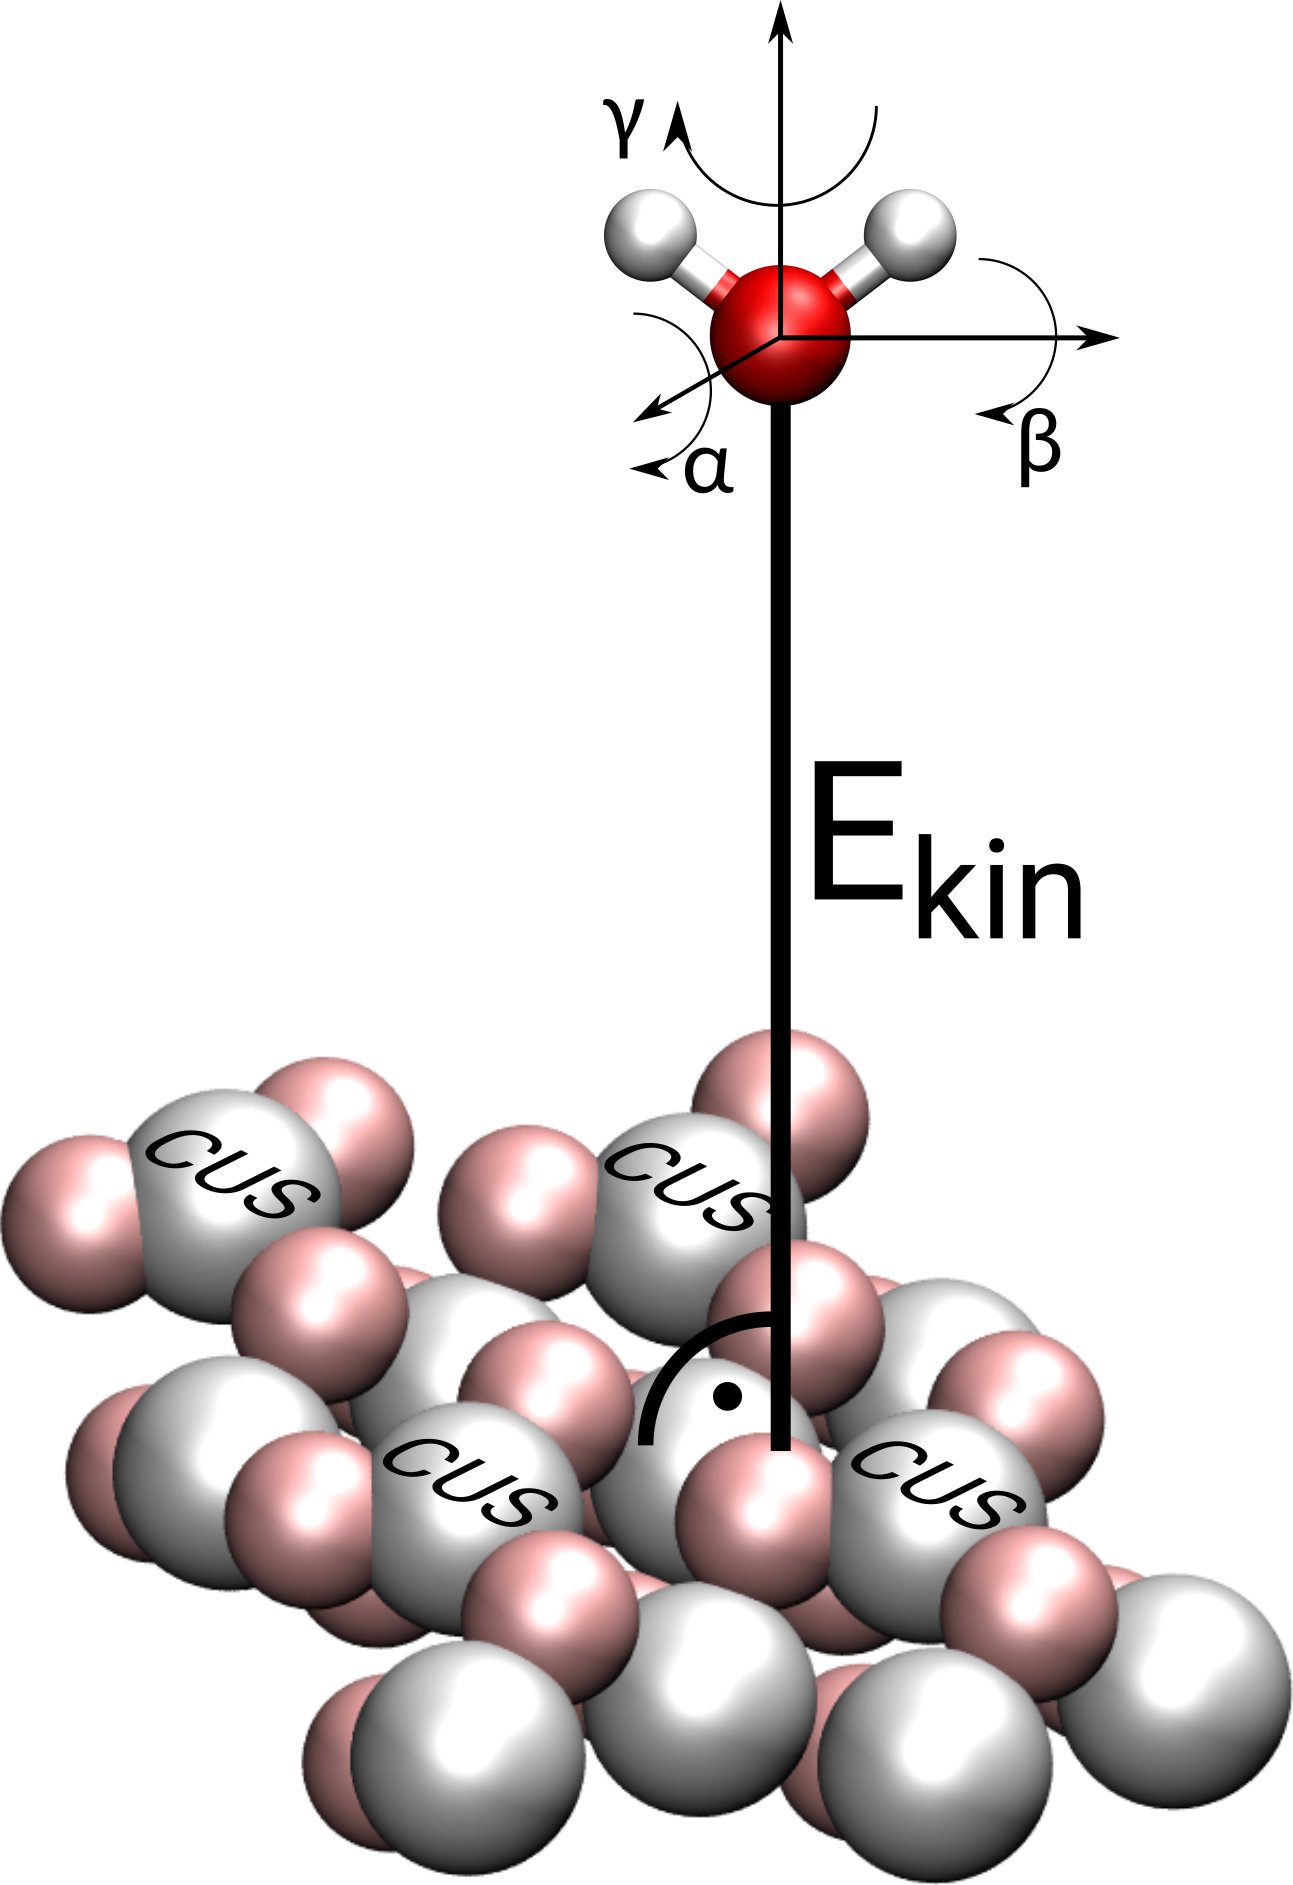
\includegraphics[width=0.5\textwidth]{figures/perspective+h2o_new.png}
\end{columns}
\end{frame}

\begin{frame}
 \frametitle{Adsorption und Dissoziationsprozess}
 Beispieltrajektorien für molekulare Adsorption, Dissoziation
 \begin{columns}
 \column{0.75\textwidth}
  \begin{figure}[h!]
  \centering
   \subfigure[molekulare Ads.]{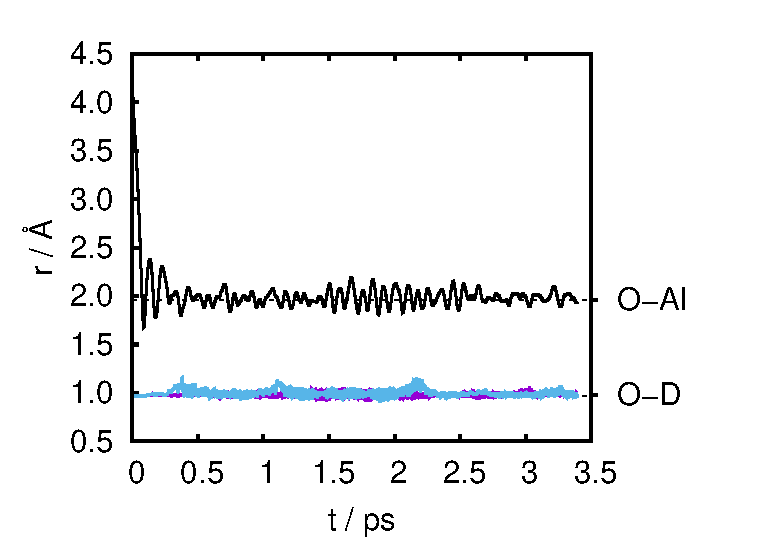
\includegraphics[width=0.4\textwidth]{figures/mol.eps}}
%    \quad
   \subfigure[1-2 Diss.]{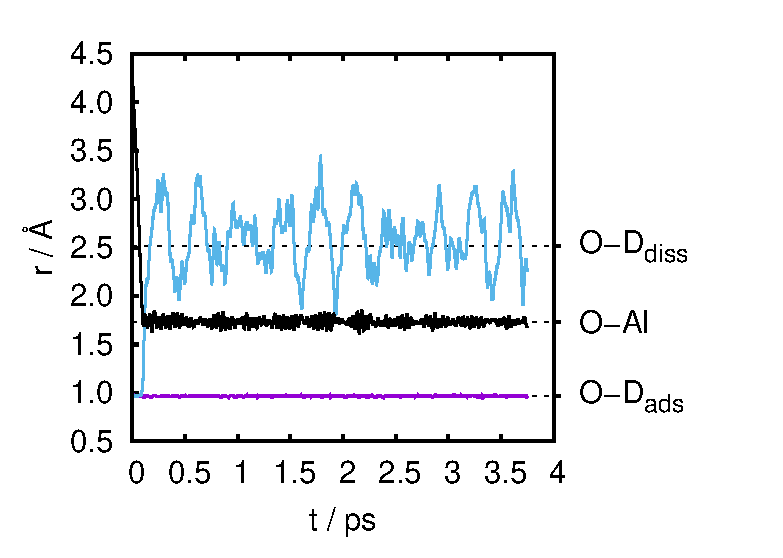
\includegraphics[width=0.4\textwidth]{figures/1-2.eps}}
 %    \quad\\
   \subfigure[1-4 Diss.]{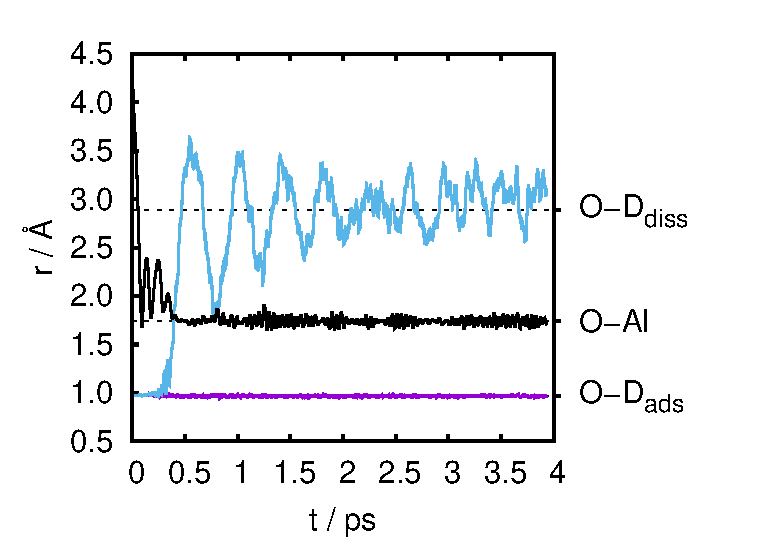
\includegraphics[width=0.4\textwidth]{figures/1-4.eps}}
%    \quad
   \subfigure[1-4$^\prime$ Diss.]{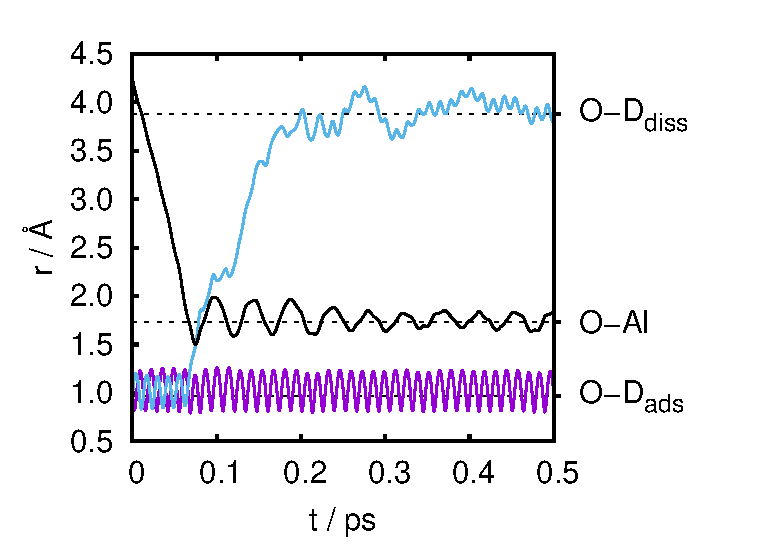
\includegraphics[width=0.4\textwidth]{figures/1-4d.eps}}
\end{figure}
\column{0.25\textwidth}
\begin{figure}
\flushleft
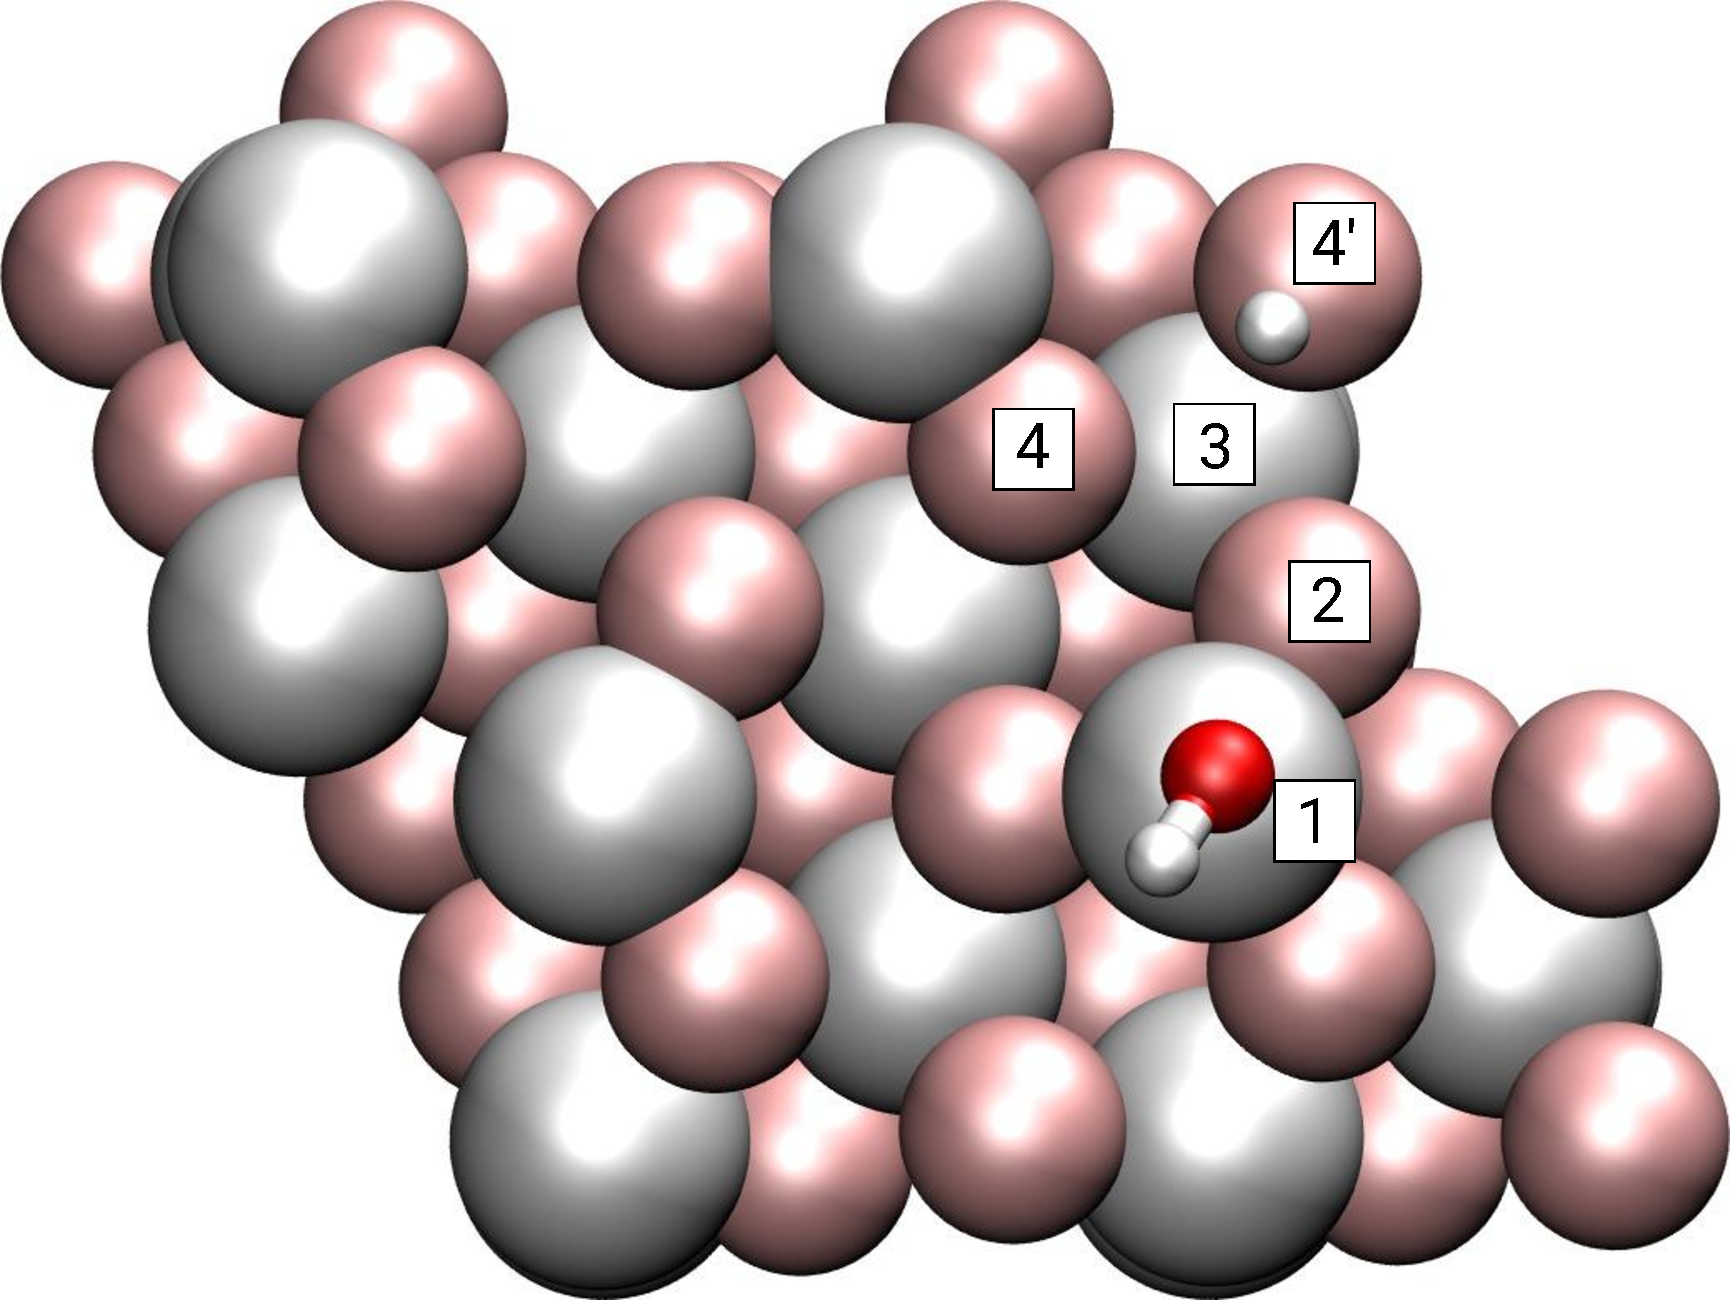
\includegraphics[width=1.\textwidth]{figures/0001_1-4p-diss_top_label.pdf}
\end{figure}
\end{columns}   
\end{frame}


\begin{frame}
 \frametitle{Dissoziations- und Adsorptionswahrscheinlichkeiten}
 \begin{columns}
 \column{0.5\textwidth}
Beispiel: Wahrscheinlichkeiten für starres Wasser, reine Oberfläche, dargestellt für Auftreffpunkte	
 \column{0.5\textwidth}
 \centering
 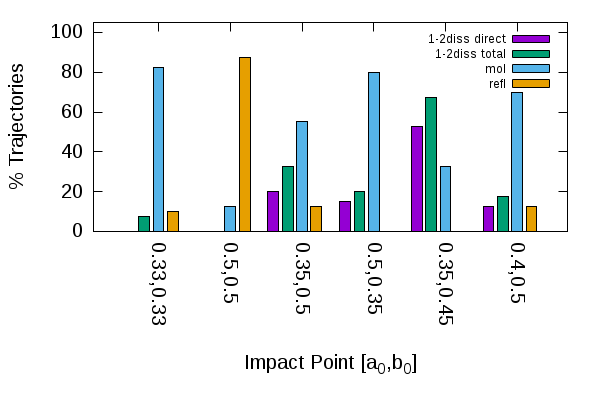
\includegraphics[width=0.9\textwidth]{figures/impactpoint.png}
%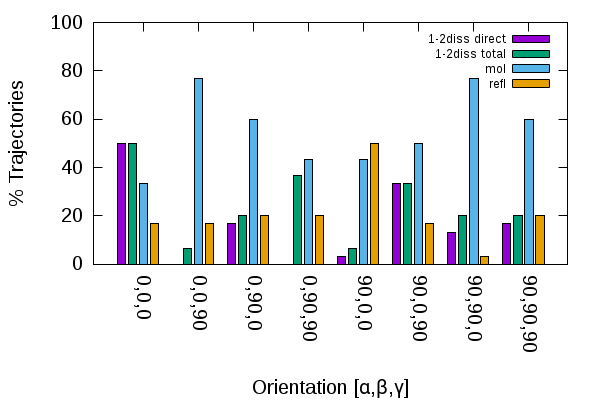
\includegraphics[width=0.45\textwidth]{figures/orientation.png}
\end{columns}
\hrule\pause
 \begin{columns}
  \column{0.5\textwidth}
  stark abhängig von
  \begin{itemize}
   \item Auftreffpunkt
   \item Temperatureffekte
   \item vorherige Bedeckung
   \item Schwingungsanregung
  \end{itemize}
% \clearpage
  \column{0.5\textwidth}
  \newline wenig abhängig von
  \begin{itemize}
   \item Orientierung des Moleküls
   \item kinetischer Energie des Strahls 
   \item $\rightarrow$ Ausnahme: Mindestenergie erforderlich
  \end{itemize}
 % \newline~\newline
 % \clearpage
 \end{columns}
\\ 
%\vspace{-.1cm}
\fbox{\parbox{0.98\textwidth}{Heiden, S.; Wirth, J.; Campen, R. K.; Saalfrank, P., \textit{J. Phys. Chem. C} \textbf{2018}, \textit{122} (27), 15494--15504.}}
\end{frame}


\section{H$_2$O@Al$_2$O$_3$(11\=20): Stabilität und Schwingungen~ ~ ~ ~ ~ ~ ~ ~ ~ ~}
\begin{frame}
 \frametitle{(11\=20) Oberfläche}
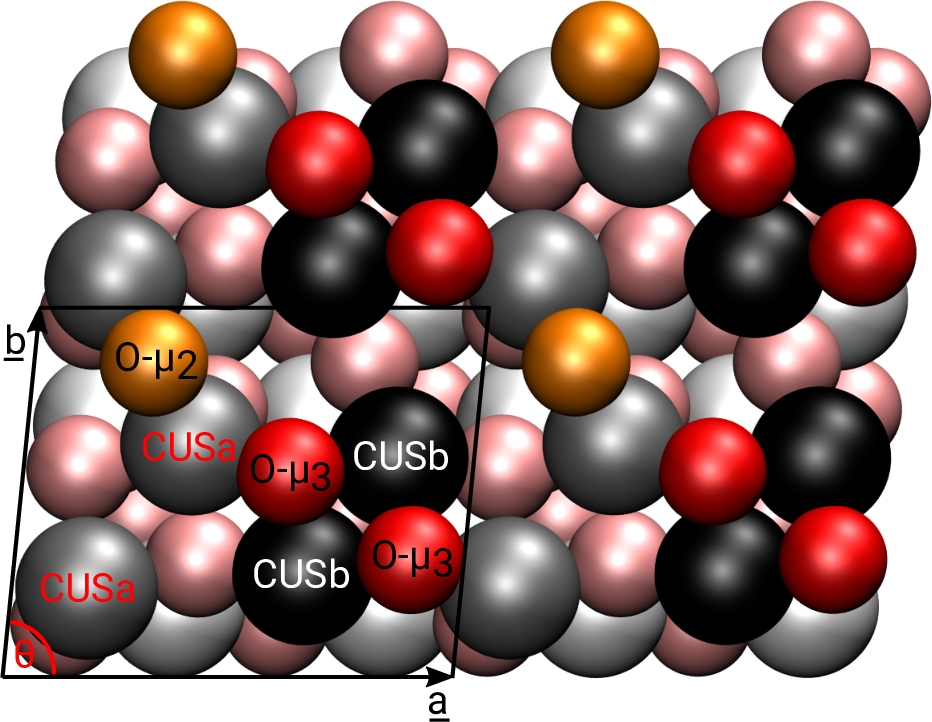
\includegraphics[width=0.4\textwidth]{figures/supercell_opt.png}~ ~ ~ ~ ~
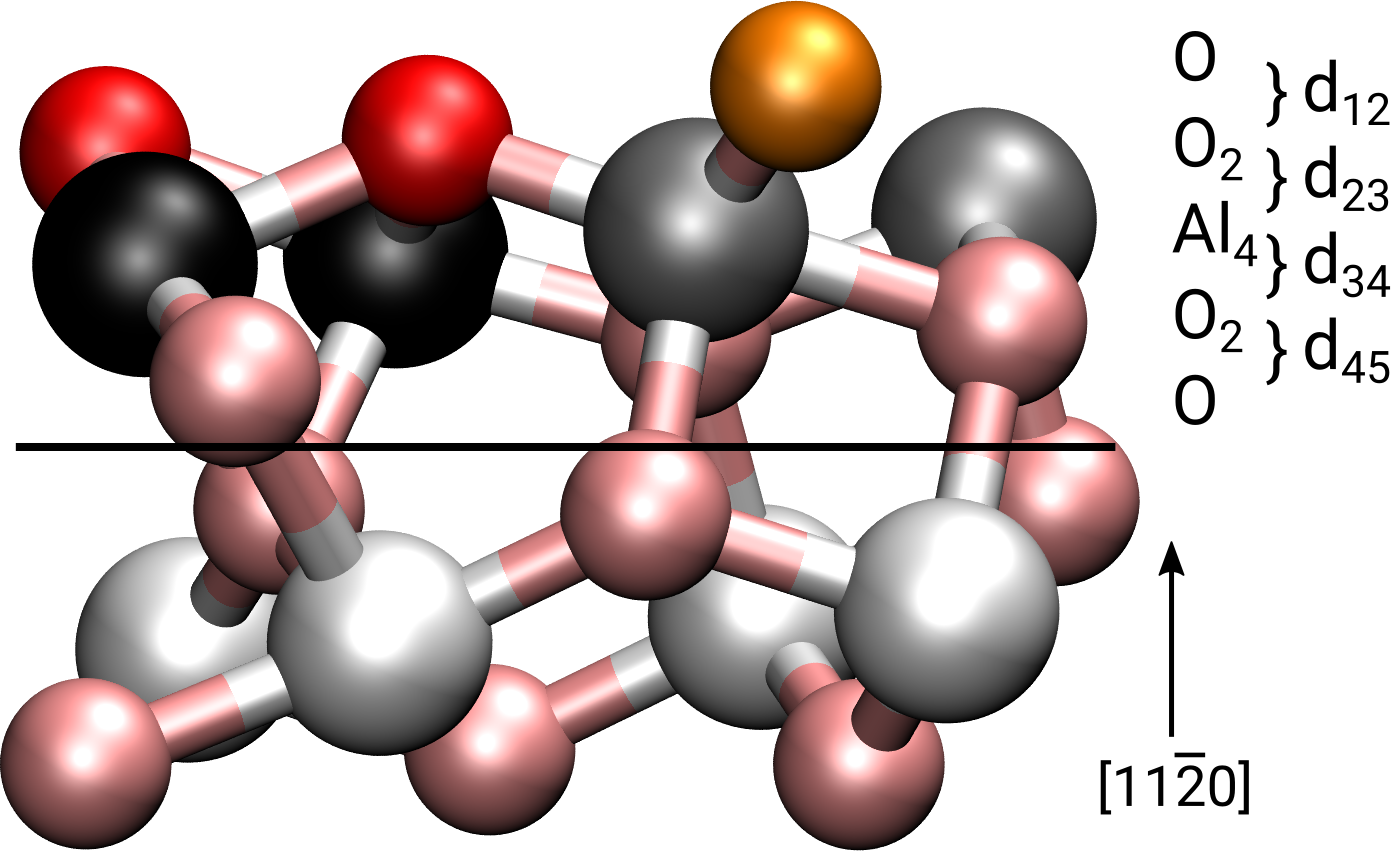
\includegraphics[width=0.4\textwidth]{figures/uc_opt.png}\\
(11\=20) Oberfläche, Draufsicht~ ~ ~~~~~~ (11\=20) Seitenansicht
\newline
 \hrule
 \begin{itemize}
  \item Optimierte Struktur (UHV $0\,$K)
 % \item O-I terminierte Oberfläche
  \item 8 CUSa und 8 CUSb Al-Atome, 8 dreifach-koordinierte und 4 zweifach-koordinierte O-Atome
  %\item ($2\times 2$) Superzelle
 \end{itemize}
 \end{frame}

\begin{frame}
 \frametitle{Wasseradsorption auf der (11\=20) Oberfläche}
 \centering
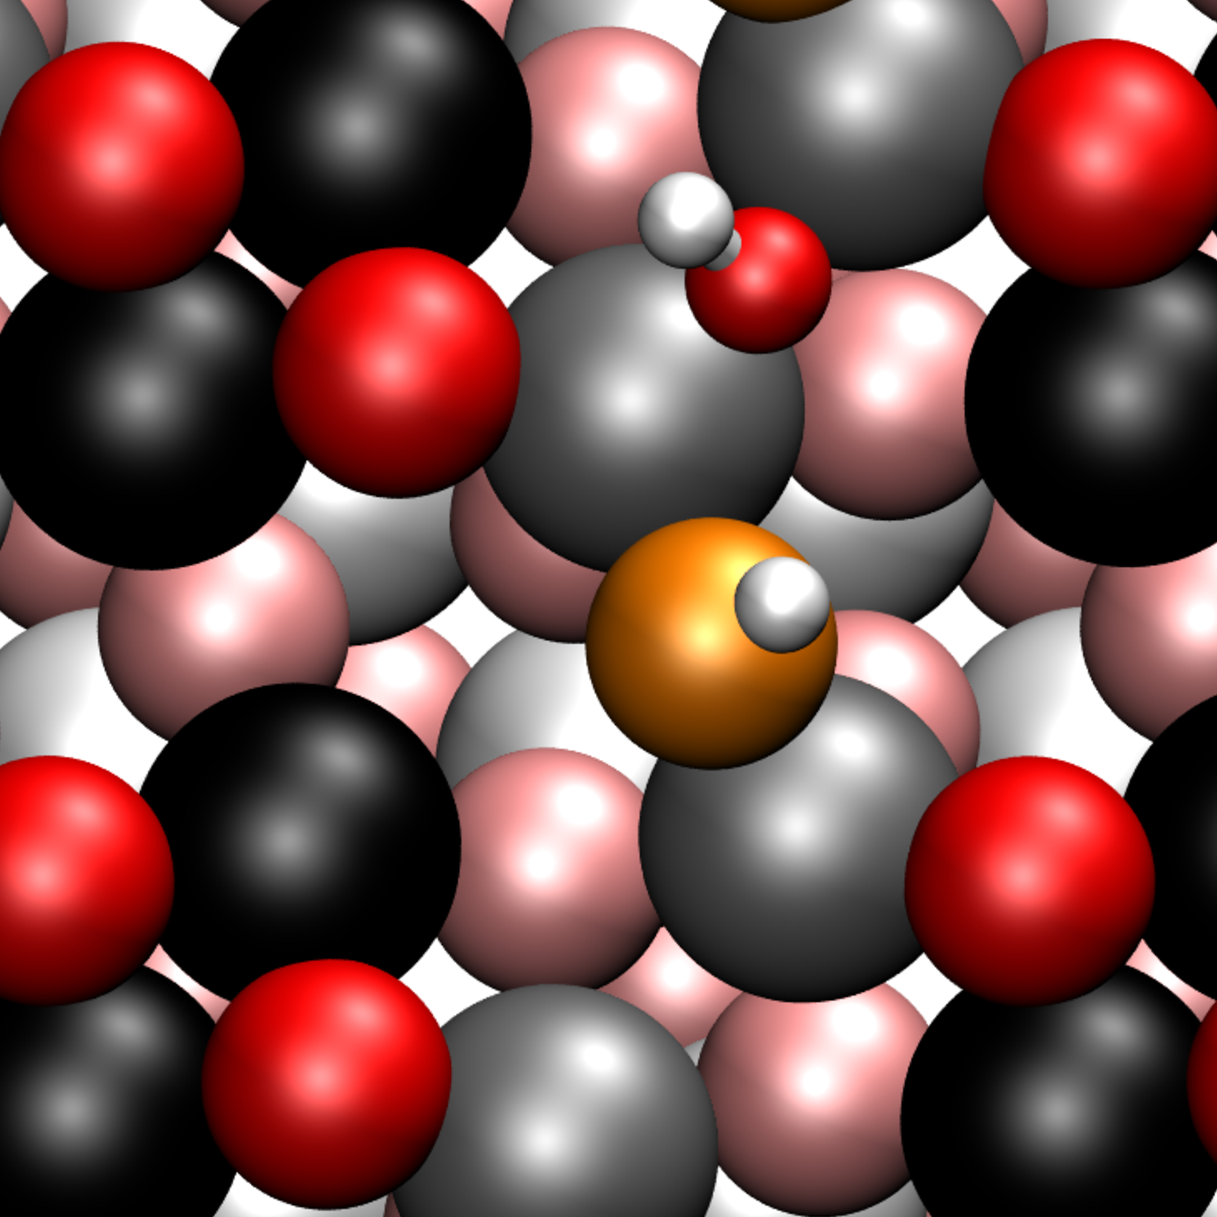
\includegraphics[width=0.25\textwidth]{figures/test-iCa2.pdf}~~~
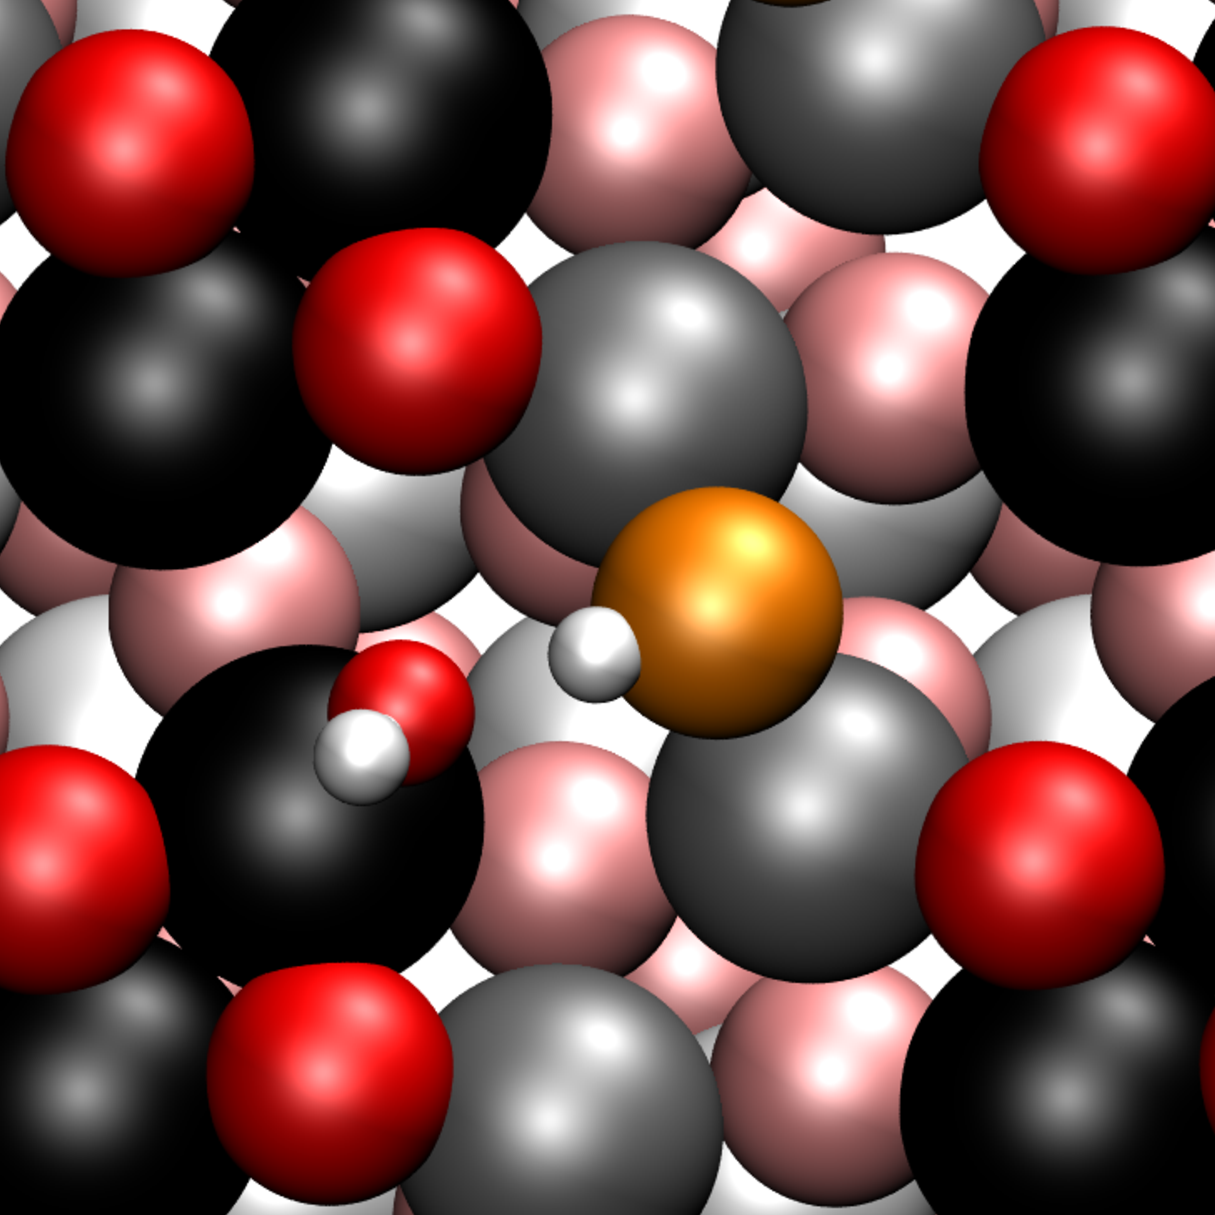
\includegraphics[width=0.25\textwidth]{figures/test-Cb2.pdf}~~~
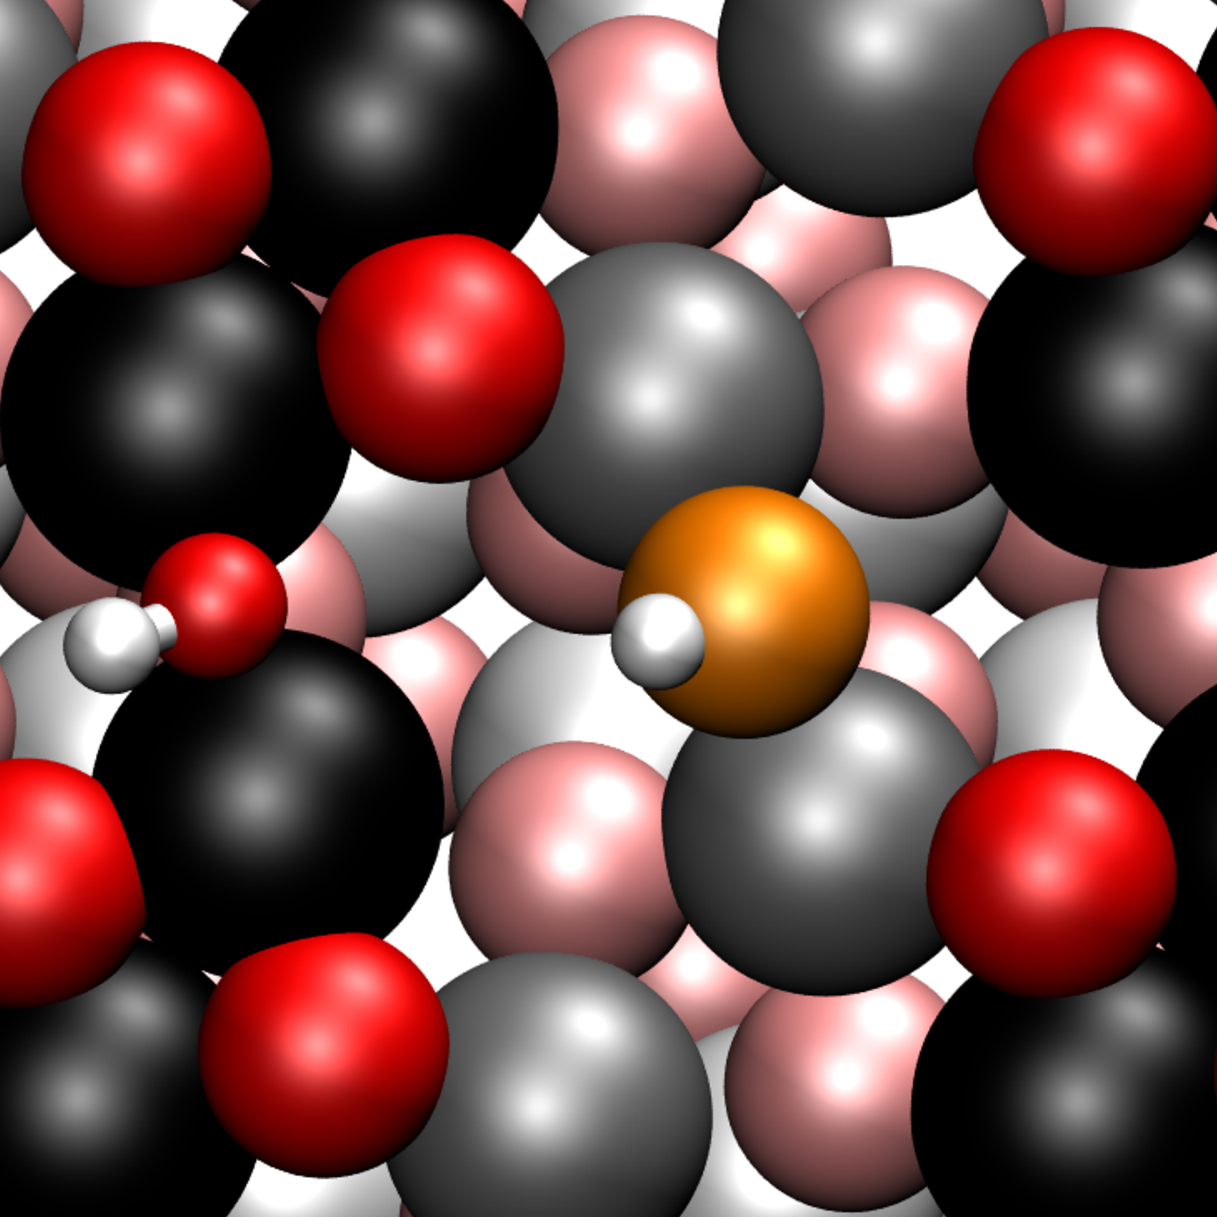
\includegraphics[width=0.25\textwidth]{figures/test-iCb2.pdf}~\newline
inter-CUSa$\parallel$O-$\mu_2$ ~~~~~CUSb$\parallel$O-$\mu_2$  ~~~~~inter-CUSb$\parallel$O-$\mu_2$~~~
\begin{table}[!ht]
  \centering
 \begin{tabular}{l|c}
  \toprule
   Adsorbierte Spezies  & $E_\textrm{ads}$  \\\midrule
 CUSb          &   -1.78   \\\hline
 inter-CUSa$\parallel$O-$\mu_2$ & \textbf{-2.50}  \\
 inter-CUSa$\parallel$O-$\mu_3$ & -1.67  \\
 CUSb$\parallel$O-$\mu_2$ & \textbf{-2.28}  \\
 CUSb$\parallel$O-$\mu_3$ & -1.19  \\
 inter-CUSb$\parallel$O-$\mu_2$ & \textbf{-2.09} \\
 inter-CUSb$\parallel$O-$\mu_3$ & -1.89 \\\bottomrule
  \end{tabular}
  \label{tab:ads_1water}
\end{table}

\end{frame}


\begin{frame}
\frametitle{Vibrationsfrequenzen der OD Spezies}
\begin{center}
  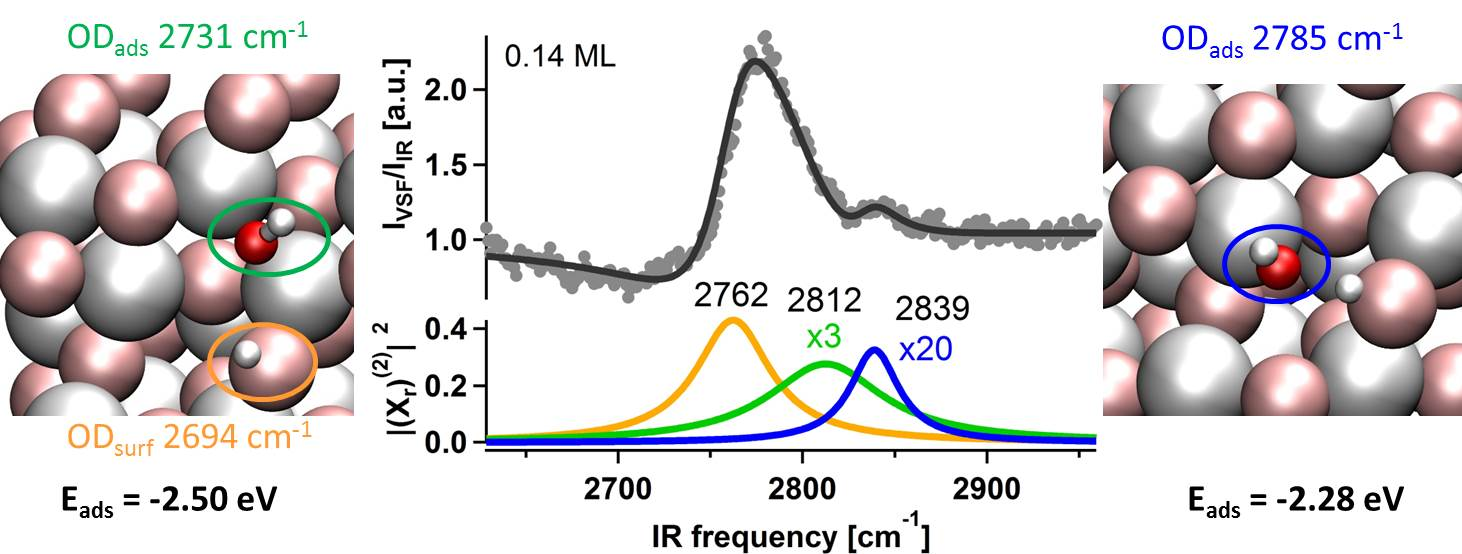
\includegraphics[width=0.75\textwidth]{figures/TOC_fig.jpg}
\end{center}
  \pause
  \vspace{-.3cm}
 \begin{table}[!h]
  \centering
  \begin{tabular}{l|ccc|cc}
%\newline
 %\caption{Wellenzahlen und Differenzen in cm$^{-1}$.}
 \toprule
 Spezies & $\tilde{\nu}_{\textrm{calc.}}$&$\Delta \tilde{\nu}_{\textrm{calc.}}$ &$\tilde{\nu}_{\textrm{exp.}}$   & $\Delta \tilde{\nu}_{\textrm{exp.}}$ [cm$^{-1}$]\\\midrule
  inter-CUSa$\parallel$O-$\mu_2$ OD$_\textrm{surf}$& 2694& & 2762& \\
  inter-CUSa$\parallel$O-$\mu_2$ OD$_\textrm{ads}$&2731 & 37 &2812 & 50\\
  CUSb$\parallel$O-$\mu_2$ OD$_\textrm{ads}$& 2785& 91 &2839 & 77 \\\bottomrule
  \end{tabular} 
\end{table}
%\newline\newline\newline
\fbox{\parbox{\textwidth}{Heiden, S.; Yue, Y.; Kirsch, H.; Wirth, J.; Saalfrank, P.; Campen, R. K., \textit{J. Phys. Chem. C} \textbf{2018}, \textit{122} (12), 6573--6584.}}
\end{frame} 
 
%\begin{frame}
%\frametitle{Vibrationsfrequenzen der OD Spezies}
% \begin{center}
%  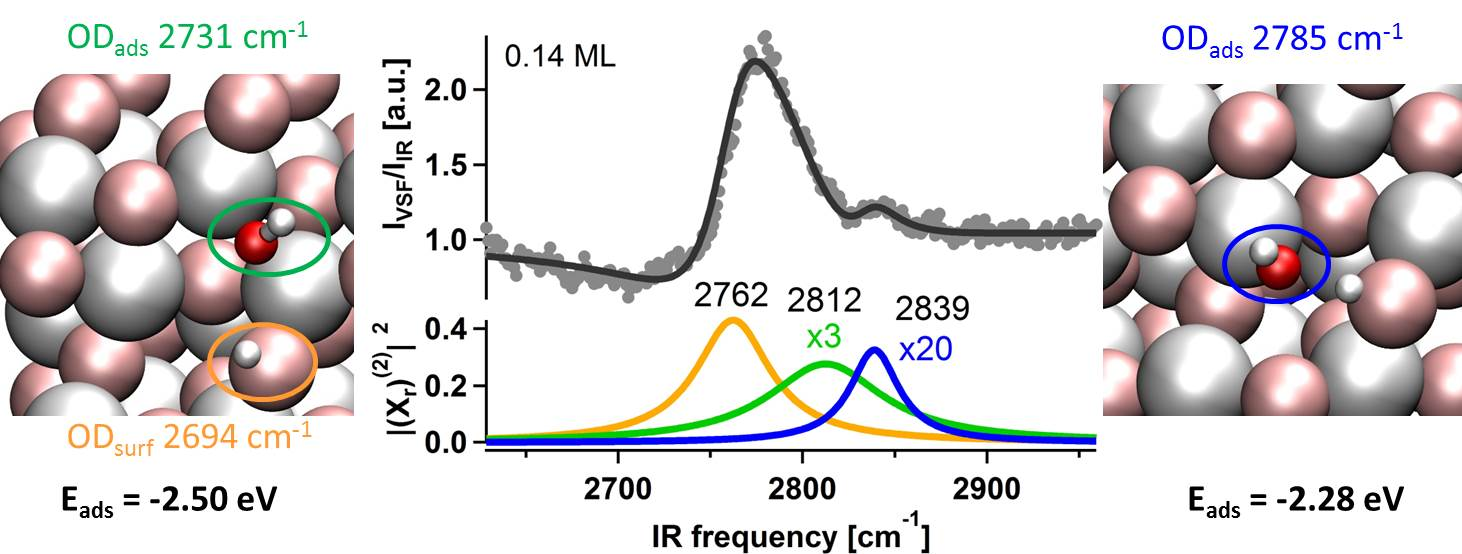
\includegraphics[width=0.75\textwidth]{figures/TOC_fig.jpg}
%  \end{center}
%\pause
%\newline~
%\begin{table}
% \begin{tabular}{l|ccc|cc}
% \caption{Wavenumbers and differences in $\tilde{\nu}$.}
% \toprule
% Spezies & $\tilde{\nu}_{\textrm{calc.}}$&$\Delta \tilde{\nu}_{\textrm{calc.}}$ &$\tilde{\nu}_{\textrm{exp.}}$ & $\Delta \tilde{\nu}_{\textrm{exp.}}$\\\midrule
%  inter-CUSa$\parallel$O-$\mu_2$ OD$_\textrm{surf}$& 2694& & 2762& \\
%  inter-CUSa$\parallel$O-$\mu_2$ OD$_\textrm{ads}$&2731 & 37 &2812 & 50\\
%  CUSb$\parallel$O-$\mu_2$ OD$_\textrm{ads}$& 2785& 91 &2839 & 77 \\\bottomrule
%  \end{tabular} 
%\end{table*}  
%\newline~\newline~\newline~
%\fbox{\parbox{\textwidth}{Heiden, S.; Yue, Y.; Kirsch, H.; Wirth, J.; Saalfrank, P.; Campen, R. K., \textit{J. Phys. Chem. C} \textbf{2018}, \textit{122} (12), 6573--6584.}}
%\end{frame} 

\begin{frame}
 \frametitle{Weitere Projekte}
 \begin{columns}
 \column{0.55\textwidth}
 \begin{itemize}
  \item Gitter Al-O Schwingungen%\newline
 \end{itemize}
 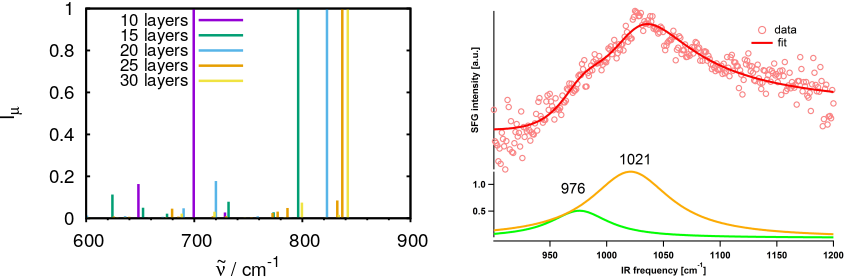
\includegraphics[width=0.9\textwidth]{figures/clean-surf-spectra.png}
 \begin{itemize}
 \item Höhere Wasserbedeckungsgrade
\end{itemize}
 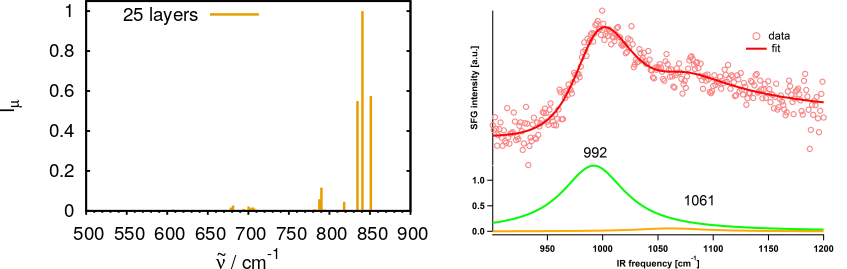
\includegraphics[width=0.9\textwidth]{figures/fully-cov-spectra.png}
 \column{0.225\textwidth}
 \begin{center}
 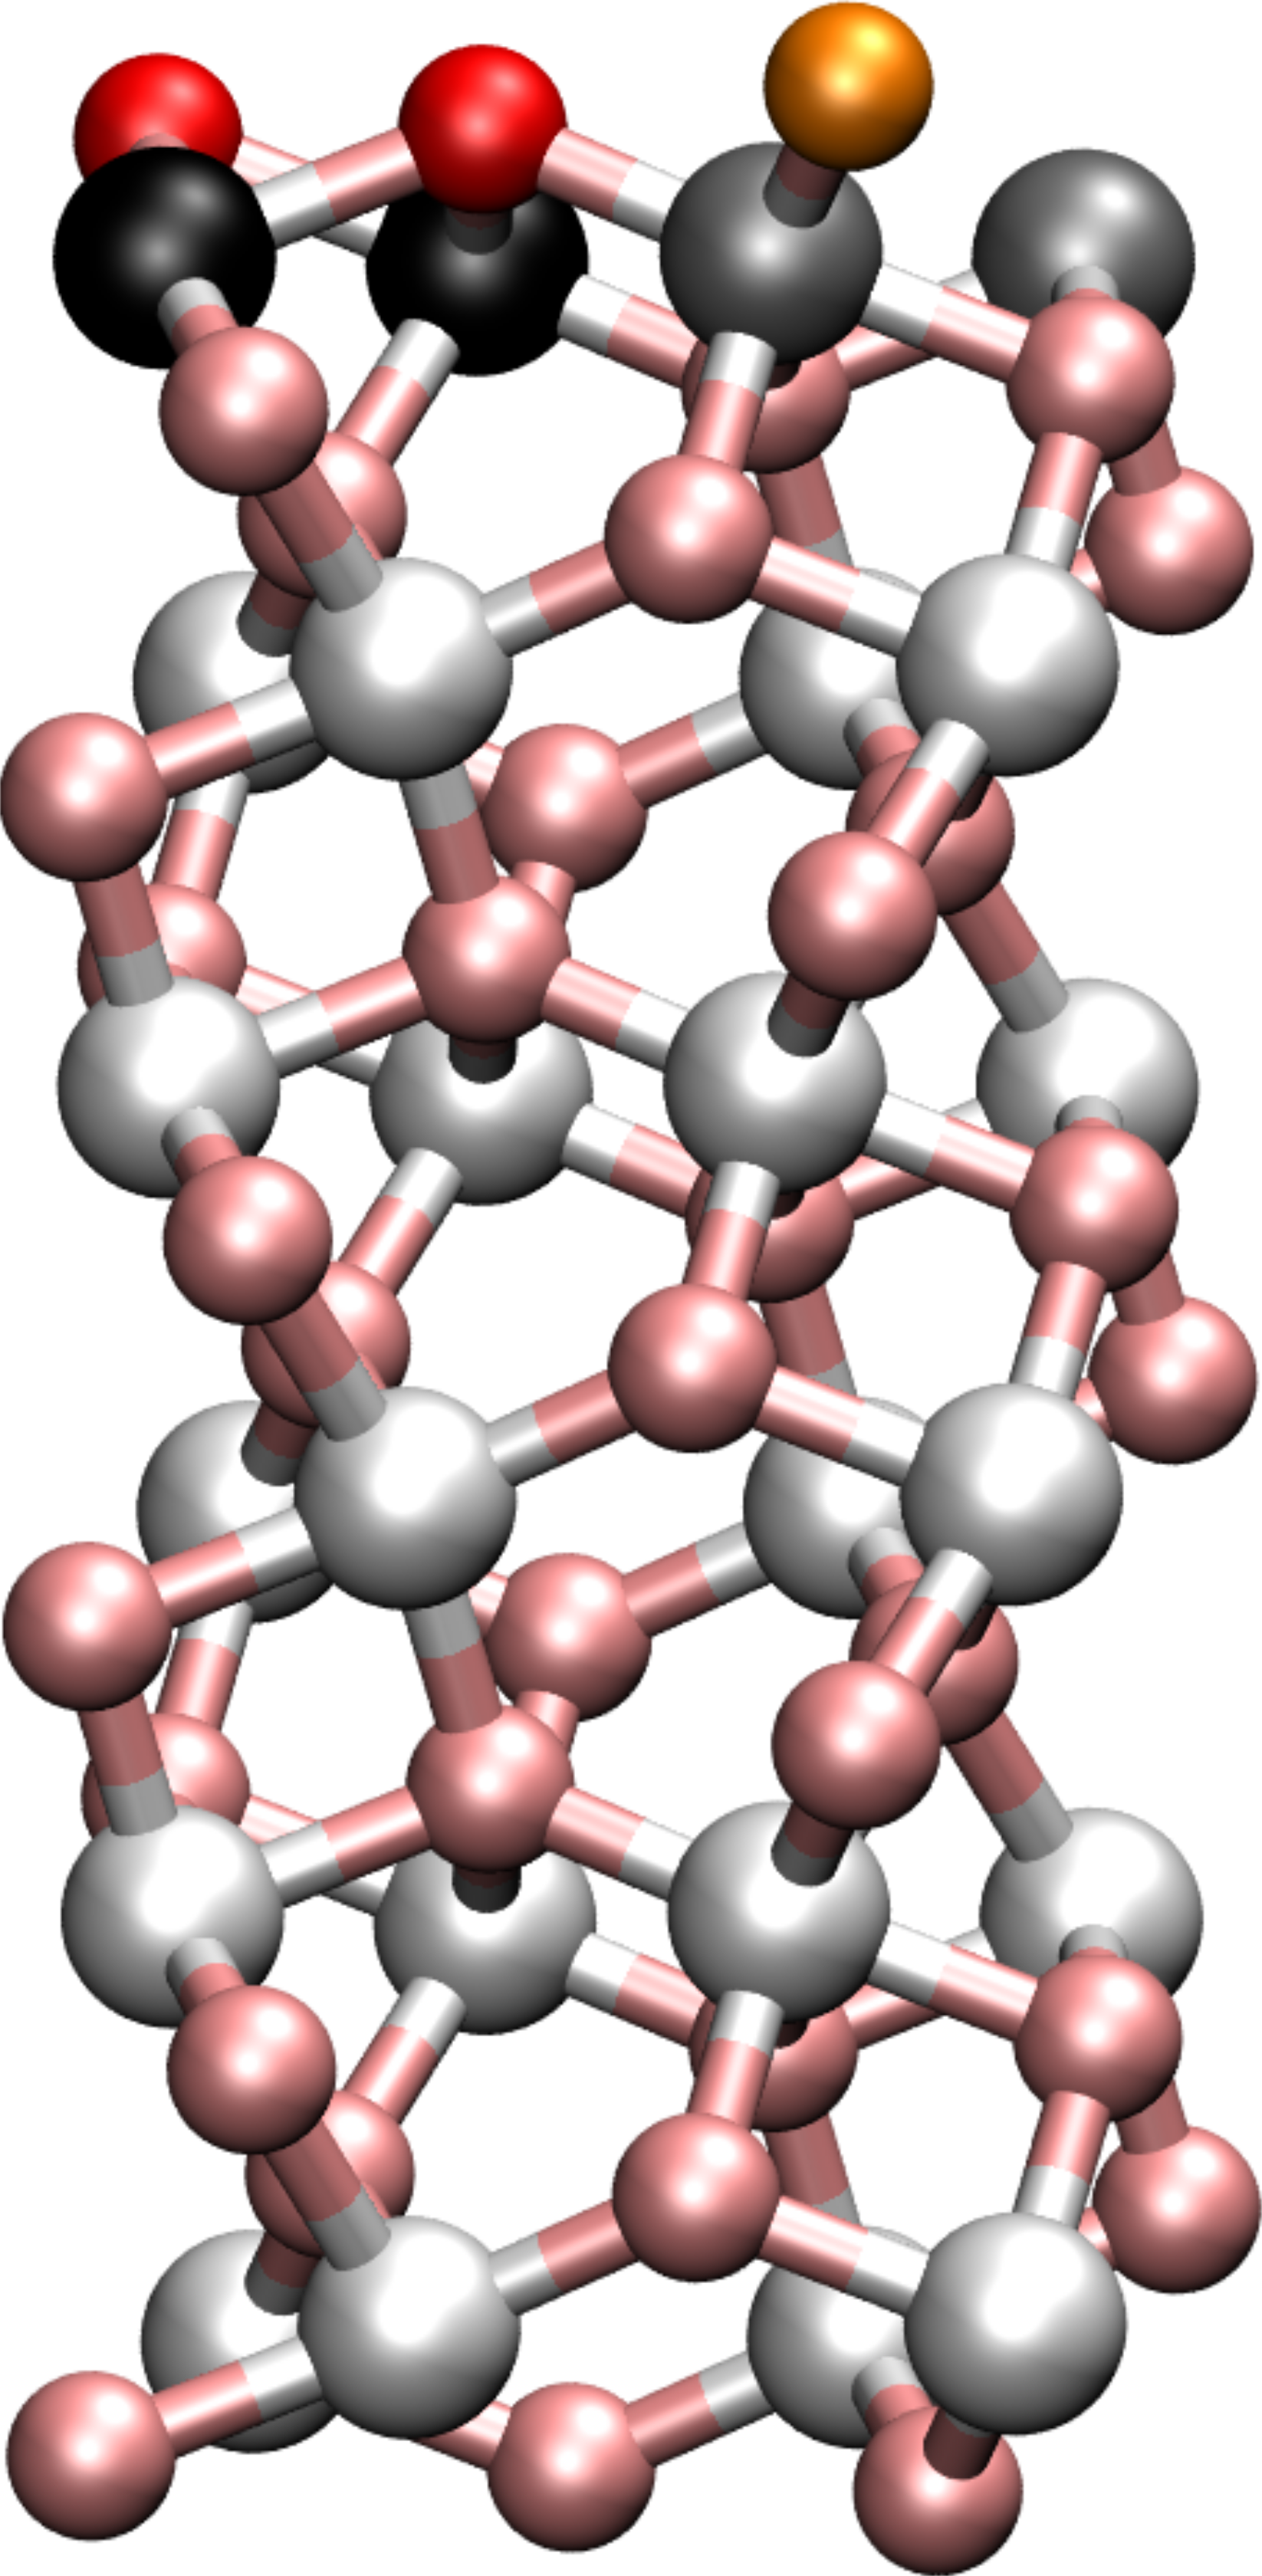
\includegraphics[width=.9\textwidth]{figures/30layer-model.png}~
 \end{center}
 \column{0.225\textwidth}
 \begin{center}
 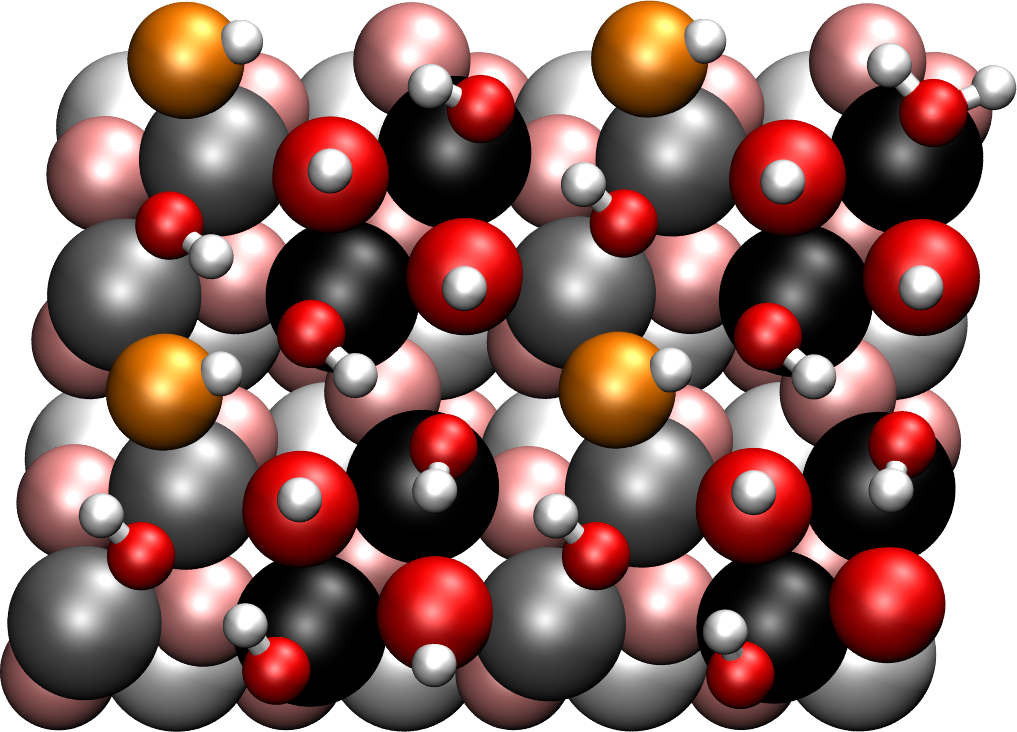
\includegraphics[width=.9\textwidth]{figures/O-I-fully.png}
 \end{center}
 \end{columns}
 \newline~\newline~\newline
\fbox{\parbox{\textwidth}{Yue, Y.; Heiden, S.; Kirsch, H.; Wirth, J.; Campen, R. K.; Saalfrank, P., in preparation}}
\end{frame}


\section*{}
\begin{frame}
 \frametitle{Zusammenfassung}
 {\color{blue}(0001) Oberfläche}
\begin{itemize}
 \item Neuberechnung von E$_{\textrm{ads}}$ 
 \item Annäherung ans Experiment bei der Berechnung von Vibrationsfrequenzen
 \item Verbesserung von Barrieren und Reaktionsraten
\end{itemize}
 \pause\hrule
\begin{itemize}
 \item MBS Experiment erfolgreich simuliert
 \item Erhöhte Dissoziation konnte verstanden werden
 \item Mechanismus der Wasseradsorption/dissoziation aufgeklärt
\end{itemize}
 \pause\hrule
 {\color{blue}(11\=20) Oberfläche}
\begin{itemize}
 \item Verhalten und Adsorptionsenergien von Wasser auf der Oberfläche
 \item Analyse der Oberflächenreaktionen
 \item Vibrationsfrequenzen von Wasser(-spezies)
\end{itemize}
 \end{frame}

\begin{frame}
 \frametitle{Danksagung}
 \begin{columns}
    \column{0.8\textwidth}
 \begin{itemize}
  \item Prof. Dr. Peter Saalfrank
  \item Prof. Dr. Beate Paulus (FU Berlin)
  \item PD Dr. Tillmann Klamroth
  \item Dr. R. K. Campen \& Yanhua Yue (FHI Berlin)
  \item Dr. Denis Usvyat (HU Berlin)
  \item AG TC, speziell: G. Melani, Dr. J. Wirth, Dr. R. W\l{}odarczyk, Spa\ss{}raum 2
 \end{itemize}
 \column{0.2\textwidth}
 \centering

\includegraphics[width=1cm]{figures/crc1109.png}
\\

\includegraphics[width=2cm]{figures/hlrn_logo.png}
\end{columns}
\centering
\includegraphics[width=8cm]{figures/ag-wise1718.png}

\end{frame}

%%%%%%%%%%%%%%ANHANG%%%%%%%%%%%%%
%\begin{frame}
% \frametitle{Adsorptionsenergien}
% \begin{table}[!h]
%  \centering
%   \caption{Adsorptionsenergien $E_\textrm{ads}$ in eV.} %der molekularen und der zwei dissoziierten adsorbierten Spezies von H$_2$O auf der Al$_2$O$_3$(0001) Oberfläche, Vergleich von plane wave Basis (PW) und Atomorbitalbasis (AO).
%   $E_{\textrm{ads}}=E_{\textrm{ads. Spezies}}-(E_{\textrm{freies Wassermolekül}}+E_{\textrm{Oberfläche}})$}
%  \begin{tabular}{ll|ccc}%c}
%  \toprule
%Basis& Methode & mol & 1-2 diss & 1-4 diss\\\midrule
%  \multirow{3}{1cm}{PW}&PW91\footnote{\textit{J. Phys. Chem. C} \textbf{116}, 26829 (2012)} %&{\color{orange}-1.25} &-1.59 &{\color{orange}-1.25} \\
%  &PW91+D2$^1$&-1.40 &-1.81 &{\color{red}-1.45} \\
%  &PBE+D2 & {\color{red}-1.31} & -1.69 & -1.21 \\
%  %&PBE+D3 &-1.29&-1.63 &-1.30 \\
%  \midrule \pause
%  \multirow{4}{1cm}{AO}&PBE+D3 &{\color{red}-1.41} &-1.68 &-1.32 \\
%  &B3LYP+D3 &{\color{red}-1.43} &-1.81 &-1.40 \\
%  &HF &-1.14 &-1.67 &{\color{red}-1.19} \\
%  &LMP2 &{\color{red}-1.34} & -1.69&-1.26\\
%  %&LMP2 (basis 9) &-1.31 &-1.61 &-1.18 \\
%  \bottomrule
%  \end{tabular}
% \end{table}
%\end{frame}

%\begin{frame}
% \frametitle{Dissoziations- und Diffusionsreaktionen}
% Eyring Gleichung: $k(T)=\frac{k_BT}{h}e^{-\Delta G^\ddagger/(k_BT)}$\newline~\newline
%\begin{table*}
%  \centering
%  \begin{tabular}{ll|cc|c}
% \toprule
%  \multicolumn{2}{c|}{\small{Reaktionstyp}}            & \small{$\Delta E^{\ddagger}$[eV]} & \small{$\Delta G^{\ddagger}(\textrm{300\,K})$[eV]} & \small{$k(\textrm{300\,K})$ [s$^{-1}$]}  \\\midrule
%\small{H$_2$O Dissoziation} &
%   \small{\textit{D-I}}  &  \small{0.01} & \small{0.002} & \small{5.76$\times 10^{12}$} \\\midrule
% \small{OH-Diffusion} &
%   \small{\textit{Df-OH-III}} &  \small{0.35} & \small{0.39} & \small{1.88$\times 10^6$}\\\midrule
%%  & \small{Df-OH-IV}  & \small{1.07} & \small{1.10} & \small{2.41$\times 10^{-6}$} \\\midrule
%\small{H-Diffusion} &
% \small{\textit{Df-H-V}}  & \small{1.65} & \small{1.49} & \small{4.90$\times 10^{-13}$} \\\bottomrule
%% & \small{Df-H-VI} & \small{1.05} & \small{0.94} & \small{1.05$\times 10^{-3}$} \\\bottomrule
%  \end{tabular}
%  \label{tab:reaction-rates}
%\end{table*}
%\centering
%\includegraphics<1>[width=0.8\textwidth]{figures/Diss_Cb-Cb2.pdf}\caption{H$_2$O dissociation}
%\includegraphics<2>[width=.8\textwidth]{figures/Diff-OH_Cb2-iCb2.pdf}\caption{OH diffusion}
%\includegraphics<3>[width=.8\textwidth]{figures/Diff-H_iCa2-iCa3p.pdf}\caption{H diffusion}
%\end{frame}


 \end{document}
